%\documentclass[a4paper, 12pt]{article}
%\documentclass[a4paper, 12pt, draft]{article} % don't include images, leave a border of same size...great
\documentclass[journal]{IEEEtran}

\hyphenation{op-tical net-works semi-conduc-tor}


%\usepackage[cmex10]{amsmath, mathtools}
\usepackage{amsmath,amssymb,amsbsy,amsfonts,amsthm}
\usepackage{multirow}
\usepackage{bm}
\usepackage{enumerate}
\usepackage{url}
\usepackage[ruled,vlined]{algorithm2e}
\usepackage{fancyvrb}
\usepackage{yfonts}

\usepackage{wrapfig}
\usepackage{tikz}
%\input{../tikz.conf}

\usetikzlibrary{bayesnet}

%%%%%%%%%%% Box 
\usepackage{calc}%    For the \widthof macro
\usepackage{xparse}%  For \NewDocumentCommand
\newcommand{\tikzmark}[1]{\tikz[overlay,remember picture] \node (#1) {};}


%% Variable de compilation
\newif\ifbeamer
\beamerfalse
\newcommand{\beamer}[2]{\ifbeamer #1 \else #2 \fi}
%%%

%\usepackage[latin1]{inputenc}
\usepackage[utf8]{inputenc} % manage utf8 encodage 
%\usepackage[english]{babel} % for french document ! dirty enumerate style,+ bad change rectangle colors for section linking.
\usepackage{fancyhdr} % for heading
\usepackage{listings}
\usepackage[colorlinks=true, urlcolor=blue]{hyperref} % url, link
\usepackage{graphicx}
\usepackage{geometry}

%\usepackage[cmex10]{amsmath, mathtools}
\usepackage{amsmath,amssymb,amsbsy,amsfonts,amsthm}
\usepackage{multirow}
\usepackage{bm}
\usepackage{enumerate}
\usepackage{url}
\usepackage[ruled,vlined]{algorithm2e}
\usepackage{fancyvrb}
\usepackage{yfonts}

\usepackage{wrapfig}
\usepackage{tikz}
    %\input{../tikz.conf}
    
\usetikzlibrary{bayesnet}
    
%%%%%%%%%%% Box 
\usepackage{calc}%    For the \widthof macro
\usepackage{xparse}%  For \NewDocumentCommand
\newcommand{\tikzmark}[1]{\tikz[overlay,remember picture] \node (#1) {};}

%%%%%%%%%% Math
\renewcommand{\text}{\textnormal}
\newcommand{\pr}{\mathbf{p}}
\newcommand{\E}{\mathbb{E}}
\newcommand{\divkk}{\mathbb{K}}
\newcommand{\entropy}{\mathbb{H}}
\newcommand{\gem}{\mathrm{GEM}}
\newcommand{\Mult}{\mathrm{Mult}}
\newcommand{\DP}{\mathrm{DP}}
\newcommand{\IBP}{\mathrm{IBP}}
\newcommand{\M}{\mathcal{M}}
\newcommand{\V}{\mathcal{V}}
\newcommand{\N}{\mathcal{N}}
    
\makeatletter
\NewDocumentCommand{\DrawBox}{s O{}}{%
    \tikz[overlay,remember picture]{
    	\IfBooleanTF{#1}{%
    		\coordinate (RightPoint) at ($(left |- right)+(\linewidth-\labelsep-\labelwidth,0.0)$);
    	}{%
    	\coordinate (RightPoint) at (right.east);
    }%
    \draw[red,#2]
    ($(left)+(-0.2em,0.9em)$) rectangle
    ($(RightPoint)+(0.2em,-0.3em)$);}
}

\NewDocumentCommand{\DrawBoxWide}{s O{}}{%
	\tikz[overlay,remember picture]{
		\IfBooleanTF{#1}{%
			\coordinate (RightPoint) at ($(left |- right)+(\linewidth-\labelsep-\labelwidth,0.0)$);
		}{%
		\coordinate (RightPoint) at (right.east);
	}%
	\draw[red,#2]
	($(left)+(-\labelwidth,0.9em)$) rectangle
	($(RightPoint)+(0.2em,-0.3em)$);}
}
\makeatother
%%%%% ! Box

\geometry{
      a4paper,
	    body={160mm,260mm},
	    left=25mm,top=20mm,
	    headheight=4mm,headsep=8mm,
        footskip=10mm,
        }
                                              

%%%%%%%%%%%%%%%%%%%%%%%%%%%%%%%%%%%%%%%%%%%%%%%%%%%%%%%%%%%%%%%%%%%%%%%%%%%%%%%%%%%%%%%%%%%%%%%%%%%%%%
%%%%% => Internal
%%%%%%%%%%%%%%%%%%%%%%%%%%%%%%%%%%%%%%%%%%%%%%%%%%%%%%%%%%%%%%%%%%%%%%%%%%%%%%%%%%%%%%%%%%%%%%%%%%%%%%

% itemize item def
%% \begin{itemize}\itemsep2pt % example space betwew item
%\renewcommand{\FrenchLabelItem}{\textbullet}
\renewcommand{\labelitemi}{$\bullet$}
\renewcommand{\labelitemii}{$\cdot$}
\renewcommand{\labelitemiii}{$\diamond$}
\renewcommand{\labelitemiv}{$\ast$}

% equation reference
\renewcommand{\theequation}{\thesection.\arabic{equation}}

%%%%%%%%%%%%%%%%%%%%%%%%%%%%%%%%%%%%%%%%%%%%%%%%%%%%%%%%%%%%%%%%%%%%%%%%%%%%%%%%%%%%%%%%%%%%%%%%%%%%%%
%%%%% => Alias
%%%%%%%%%%%%%%%%%%%%%%%%%%%%%%%%%%%%%%%%%%%%%%%%%%%%%%%%%%%%%%%%%%%%%%%%%%%%%%%%%%%%%%%%%%%%%%%%%%%%%%

% write code
\lstnewenvironment{C}[1]
{\lstset{language=C,
      frame=tBRl,
      basicstyle=\scriptsize,stringstyle=\emph,showstringspaces=false,
      numbers=left,numberstyle=\tiny,
      breaklines=true, columns=flexible, title={#1}}
}{}
      
%%%%%%%%%%%%%%%%%%%%%%%%%%%%%%%%%%%%%%%%%%%%%%%%%%%%%%%%%%%%%%%%%%%%%%%%%%%%%%%%%%%%%%%%%%%%%%%%%%%%%%
%%%%% => Preambles Pages
%%%%%%%%%%%%%%%%%%%%%%%%%%%%%%%%%%%%%%%%%%%%%%%%%%%%%%%%%%%%%%%%%%%%%%%%%%%%%%%%%%%%%%%%%%%%%%%%%%%%%%

\pagestyle{fancy}
\fancyhf{} % remove default headers
\fancyfoot[C]{\thepage}
\renewcommand{\footrulewidth}{0.3pt}
\renewcommand{\headrulewidth}{0.3pt}

%%%%%%%%%% Math
\renewcommand{\text}{\textnormal}
\newcommand{\pr}{\mathbf{p}}
\newcommand{\E}{\mathbb{E}}
\newcommand{\divkk}{\mathbb{K}}
\newcommand{\entropy}{\mathbb{H}}
\newcommand{\gem}{\mathrm{GEM}}
\newcommand{\Mult}{\mathrm{Mult}}
\newcommand{\DP}{\mathrm{DP}}
\newcommand{\IBP}{\mathrm{IBP}}
\newcommand{\M}{\mathcal{M}}
\newcommand{\V}{\mathcal{V}}
\newcommand{\N}{\mathcal{N}}
    
\newcommand{\mat}[1]{\mathbf{#1}}

\title{Are latent feature/class models adapted for link prediction in social networks?}

%\date{avril 2015}

\newtheorem{definition}{Definition}[section]
\newtheorem{proposition}{Proposition}[section]
\newtheorem{theorem}{Theorem}[section]

\begin{document}
	
\maketitle
\begin{abstract}
\end{abstract}

\IEEEpeerreviewmaketitle



\section{Introduction}
\label{sec:introduction}
In recent years, several powerful relational learning models have been proposed to solve the problem commonly referred to as \textit{link prediction} that consists in predicting the likelihood of a future association between two nodes in a network \cite{Liben-Nowell07, HassanZaki11}. Among such models, the class of probabilistic, generative models has received much attention as such models can be used to both generate artificial networks and infer new links from existing ones. Two main class of models have been proposed and studied in the literature: the latent feature model \cite{BMF} and its non-parametric extension \cite{ILFRM}, and the mixed-membership stochastic block model \cite{MMSB} and its non parametric extensions \cite{iMMSB,diMMSB}. In this paper, we focus on this two model, and study some of its properties related to link prediction in social networks. 

Indeed, although drawn from a wide range of domains, most real world social networks exhibit common properties, such as the \textit{homophily}, \textit{preferential attachement} and \textit{small world} effects \cite{Newman2010, Barabasi2003}. 


A natural question that arises is thus whether or not models as IMMSB and ILFM comply with such properties. Link prediction model, typically learned or given, describe a set of nodes and links between them; Such data defines a random structure $Y$. Given that, we learn a model parameters $\hat \theta$, such that one can then predict the probability that a new link will be drawn between two given nodes of the network by studying the following quantity:
\begin{equation}
\p(y | \hat \theta)
\end{equation}
This quantity is called a predictive likelihood.


A question we ask in this setting is: \textit{Do link prediction models learned can generate networks with the homophily and preferential attachment}.

A second possible use of Bayesian models is as a pure generative model to generate artificial networks. In this setting, we study models properties based on their expectation over their random parameters, defined as follows:

\begin{equation}
\p(y) = \int_{\theta} \p(y,\theta) d\theta
\end{equation}
This quantity is know as the evidence for the data.

The question we ask ourselves in this setting is thus: \textit{Do link prediction models comply with the homophily and preferential attachment effects}.


The remainder of the paper is organized as follows. In the second section \ref{sec:background} we set up the probabilistic context of our analysis, Then in section \ref{sec:models} we present two general class of models in this settings know as class based models and feature based models. Then in section \ref{sec:homophily} and \ref{sec:burstiness} we propose respectively formal definition for the homophily and preferential effects and study how models comply with this propoerties. \textcolor{red}{Then section on feature dynamics and sparsity}. In section \ref{sec:experiments} we report an empirical study of the predictive performance on synthetic and real networks with regards to the properties. We conclude in the last section \ref{sec:concl}. 

%\section{Motivations}
Recently, several complex Bayesian models based on latent variables have been used to explain the structure of social networks [mmsb, ilfrm, etc]. Those studies was mainly evaluated on prediction tasks, such as link prediction or communities detection. However, few works have been done concerning the study of the intrinsic capacity of the models to model basic properties that arise in social networks, such as the dynamics of degree distribution, known to exhibit the preferential attachment effect [barabasi, web..] or the homophily effect[ref].
% For exemple, the heavily study Latent Dirichlet Allocation Model LDA model, being a particular of Mixed Membership Stochastic Blockmodel (MMSB) for networks, made no epistomological claim about the conjugacy used. In this work we found that conjugacy played a role in the ability of the model to capture some properties.
~\\


(++ Indeed the most heavily studied properties in social networks was the degree distribution and the mixing pattern (homophily/assortativity) tableaux !)

(++ not clear consensus of the formalism of properties and their evaluation, and whatsoever for the homophily property, the feature the definition are usually for single attribute... We consider a general vector . (with a measure working for both latent and real features)

(++ Probabilistic models we are interested in provide two ways of representing the data or network. One fall in the paradigm of mixture models and the other in the latent feature modeling. A motivation of those two modeling paradigm is that they are consistent with two key nonparametric prior for discrete data, namely the Dirichlet process (DP) and the the Indian Buffet Process (IBP). Many baysian model can be view as equivalent to truncated models with nonparametric priors. This provide a motivation to study those models. Furthermore, they are used as priors to generate latent features, either as proposition vector (class/DP) or binary vector (feature/IBP). It is admitted that those priors gives bursty features [accounting for burstiness in topic model]. We seek to clarify why this is true and how the burstiness can propagate at the degree level.~\\


In the next section we will, first, explain the mathematical background in a machine learning context. Secondly, we will review the models of interest for dyadic data. Then, we will introduce the formal definition of properties of interest in social networks within the Bayesian frameworks, and how this is translated in terms of assumptions within Bayesian priors. Finally, we will show empirical results (on synthetic and real datasets) to support our claims.~\\

%Study the poisson binomial distribution for the out links of a node. This is the degree distribution and should be bursty to have community in networks.


\section{Latent Representation}
\label{sec:background}
Without loss of generality, we focus on social networks with binary relationships. A network with $N$ nodes is a graph $G = (V,E)$, where $V$ is a set of nodes (typically representing entities) and $E \in V \times V$ is a set of edges between nodes (typically representing relationships between pairs of entities).The topology of the network is described by the presence or absence of links between nodes in the graph, and can be represented by an adjacency matrix $Y \in \{0,1\}^{N\times N}$.\\

For the link prediction problem in social networks, there is two main approach found in the machine learning literrature. One based on matrix factorization \cite{menon2011link} and the other based on probabilistic models \cite{goldenberg2010survey}. While the former approach often lead to optimization algorithms that scale better, the second offer a richer expressivness and data explanation power, it worth to say that, as for PLSA method, it is always possible to normalize matrices to view the factorization problem as a a probabilistic model. But a deeper relation exists which highlight similarities and differences between both representations. It is due the the assumptions of exchangeability that we make on data, that we expose now.\\

Let's consider the parameters of a network model consisting of a tuple $\Theta = \{ \mat{F} , \mat{\Phi}\}$ such as $\mat{F} \in \mathcal{F}^{N\times K}$ is a matrix representing the latent features of nodes and $\mat{\Phi} \in \mathcal{W}^{K\times K}$ a matrix of weight interactions. The learning problem consist in finding the best model parameters given some criterion to reconstruct the data such as $Y \approx \mat{F}\mat{\Phi}\mat{F}^T$. In matrix factorization, we optimize the following criterion which relate to an empirical error minimization:
\begin{displaymath}
    \min\limits_{\Theta} \frac{1}{|Y|} \sum_{(i,j) \in Y} \ell(y_{ij}, \hat y_{ij}(\Theta)) + \mathcal{R}(\Theta)
\end{displaymath}
Where $\ell$ is a loss function and $\cal R$ a regularisation term.

In probabilistic modelling, the learning problem is to find the posterior distribution $\p(\Theta | Y)$. Additionnaly, because we focus on static networks here, we make the assumptions of jointly exchangeable graph. It means that the order in which we oberve nodes does not matter. Under such assumptions, the Haldoos-Hoover representation theorem \cite{orbanz2015bayesian}, tell us that the likelihood of the model that we consider has a factorial distribution such as $\p(Y | \Theta) = \prod_{(i,j) \in Y} \p(y_{ij}| \Theta)$. In this settings, the criterion to optimze relate to the maximum a posteri (MAP): 
\begin{displaymath}
    \max\limits_{\Theta}  \frac{\p(Y | \Theta) \p(\Theta)}{\p(Y)}
\end{displaymath}

By taking the log of the MAP, it is easy to show that it is equivalent to optimize the following criterion:
\begin{displaymath}
    \min\limits_{\Theta} \sum_{(i,j) \in Y} \left( \log(\p(y_{ij})) - \log(\p(y_{ij}|\Theta))\right) - \log(\p(\theta))
\end{displaymath}


This form hilights the equivalence between the matrix and the probabilistic representation. Indeed, one see that the loss fonction become the error between the log-evidence and the log-likelihood and the regularization term is equal to the negative of the log prior.


Finally, because we model binary retionship, a natural kernel for the observation is a bernoullli density, thus we have the following matrix representation for the likelihood:
\begin{equation}
E_{y \sim p(y \mid \Theta)}[Y] = \mat{F} \mat{\Phi}  \mat{F}^T
\end{equation}

This formalism is similar to work of Buntine on Discrete Component Ananlysis(DCA) \cite{DCA}. In the following we will study two particular models (iMMSB ILFM), that refers to mixed membership model in the sense that the likelihood of the models are defined as a mixture of membership such as:
\begin{equation}
\pr(y_{ij}=1 \mid \Theta ) = \sum_{k, k'} \pr(y_{ij}=1\mid\phi_{k,k'}) \pr(k \mid \mat{f}_i) \pr(k' \mid \mat{f}_j)
\end{equation}

%See the Appendix~\ref{sec:mixmembership} for a justification of eq \eqref{eq:mf} using a Mixed Membership Model approach.
A key point here, is that the Stochatistic Blockmodel well studied in the literrature \cite{goldenberg2010survey}, where nodes of the networks belong only one clusters (blockmodel) is a special case of this formalism (as well as MMSB and ILFM for extrem case) when the feature vector $f_i$ of node $i$ has one element corresponding to the membership while other are zeros. Besides the choice of prior on $\Phi$ and $\Theta$ represent the context in which  their elements can evolve.

In this framework, we want to answer the following questions:
\begin{itemize}
	\item What properties the model can capture or learn on networks ?
	\item Which constraint on the models can come with an consistent interpretation of latent variables along with the concepts of communities structure and homophily in social networks  ?
\end{itemize} 

%%%

In the next session we review both iMMSB and ILFM more precisely.


\section{Models}
%\emph{Yet another view} ~\\
\label{sec:models}

As mentioned before, we focus in this study on two major representatives of the latent models used for link prediction in social networks, namely the latent feature model \cite{BMF} and the mixed-membership stochastic block model \cite{MMSB}. To be as general as possible, we consider non-parametric extensions of these models, respectively based on the Indian Buffet Process (IBP) and the Hierarchical Dirichlet Process (HDP). Similar extensions have already been considered in the past, {\it e.g.} through the Infinite Latent Feature model \cite{ILFRM} and through conditional random fields \cite{iMMSB} or a dynamic version of the Hierarchical Dirichlet Process \cite{diMMSB}.
%\textcolor{red}{To be completed - maybe second extension not considered yet}

We now briefly describe the two models retained.
%Our two chosen baseline use prior distributions that fall into the two major classes of discrete nonparametric priors. The Hierarchical Dirichlet Process (HDP) that generalizes the Latent Dirichlet Allocation (LDA) for infinite mixtures models. On the other hand, the Indian Buffet Process (IBP), which is the generalization of the Beta-Bernoulli compound distribution (ie Beta Process), which generates infinite binary matrices. The nonparametric models in their truncated version are equivalent to well-known models such as LDA, widely used for text analysis, and Mixed Membership Stochastic Blockmodel which is an adaptation of the latter for relational learning.~\\

%We adopt the following notation; if a matrix has a negative index superscripted, it indicates that the values corresponding to this index are excluded. A dot $\bm{.}$ in the index means that we marginalize over all possible values.

\subsection{Infinite Latent Feature Model (ILFM)}

In the latent feature model, each node is represented by a vector of binary features. The probability of linking two nodes is then based on a weighted similarity between their feature vectors, the weight matrix being generated according to a normal distribution. In its non-parametric version, the feature vectors are now generated according to an IBP, leading feature vectors of infinite dimensions (even though only a finite number of dimensions are actually active). The following steps summarizes this process:
%
\begin{enumerate}
\item Generate a feature matrix $\mat{F}_{N \times \infty}$ representing the feature vector of each node: $\mat{F} \sim \IBP(\alpha)$
\item Generate a weight matrix for each latent feature:\\
 $\mat{\phi}_{mn} \sim N(0, \sigma_w), \, m,n \in \mathbb{N}^{+*}$
\item Generate or not a link between any node $i$ and any node $j$ according to: 
%
\begin{equation}
y_{ij} \sim \mathrm{Bern}(\sigma(\mat{f}_{i} \mat{\Phi} \mat{f}_{j}^\top))
\label{eq:link-ilfm}
\end{equation}
\end{enumerate}
%
where $\sigma()$ is the sigmoid function, mapping $[-\infty, +\infty]$ values to [0,1], and where $y_{ij}$ is a binary variable indicating that a link has been generated ($y_{ij}=1$) or not ($y_{ij}=0$). We will denote by $\mat{Y}$ the $N \times N$ matrix with elements $y_{ij}$. Finally, $\mat{f}_{i}$ denotes the row vector corresponding to the $i^{th}$ row of $\mat{F}$.

This model makes use of two real hyper-parameters, one for the IBP process ($\alpha$), and one for the variance of the normal distribution underlying the weight matrix ($\sigma_w$). In the case of undirected networks, the matrices $\mat{Y}$ and $\mat{\Phi}$ are symmetric and only their upper (or lower) diagonal parts are generated. Lastly, both $\mat{F}$ and $\mat{\Phi}$ are infinite matrices. In practice however, one always deal with a finite number of latent features. A graphical representation of this model is given in Figure~\ref{fig:ilfrm}.

\begin{figure}[t]
	\centering
	\minipage{0.25\textwidth}\vspace{1cm}
	\scalebox{0.88}{
	\begin{tikzpicture}
  % Define nodes
  \node[obs]                      (y) {$y_{ij}$};
  \node[latent, left=1.2cm of y] (fi) {$\mat{f}_i$};
  \node[latent, right=1.2cm of y] (fj) {$\mat{f}_j$};
  \node[latent, above= of y]    (ibp) {$\mat{F}$};;
  \node[latent, below= of y, yshift=-0.3cm]   (W) {$\mat{\Phi}$};
  \node[const, left=0.7cm of ibp]   (a) {$\alpha$};
  \node[const, right=0.7cm of W]   (sw) {$\sigma_w$};

  % Connect the nodes
  \edge {fi,fj,W} {y} ;
  \edge[dashed] {ibp} {fi,fj} ;
  \edge {sw} {W} ; 
  \edge {a} {ibp} ; 

  % Plates
  \plate {yx} {(fj)(y)} {$N$} ;
  \plate[label={[label distance=-0.6cm]195:$N$}] {} {(fi)(y)(yx.north west)(yx.south west)} {} ;
  %\plate {} {(W)} {$K\times K$};
  %\plate {} {(fi)(y)(yx.north west)(yx.south west)} {$N$} ;
\end{tikzpicture}
}
	\endminipage
	\minipage{0.25\textwidth}
	\scalebox{0.88}{
		/home/dulac/Documents/workInProgress/networkofgraphs/papers/personal/figures/draw/mmsb2.tex}
	\endminipage
	\caption{The two graphical representations of (left) the latent feature model and (right) the latent class model. The difference between the two models lies in the way representations are associated to nodes: a fixed representation is used in the case of the latent feature model, whereas the representation in the latent class model varies according to the link considered.}
	\label{fig:ilfrm}
\end{figure}

Standard Gibbs sampling and Metropolis-Hastings algorithms can be used for inference in this model. We do not detail them here and refer the interested reader to \cite{ILFRM}.

%We here only provide the main updates, useful for the developments presented in the next sections, and refer the reader to \cite{IBP} for a detailed treatment. The Gibbs update for the matrix $\mat{F}$ are given by:
%%
%\begin{align}
%& P(f_{ik} = 1 \mid \mat{F}^{-ik}) = \frac{m_k^{-i}}{N} \nonumber \\
%& P(f_{ik} = 0 \mid \mat{F}^{-ik}) = 1 - \frac{m_k^{-i}}{N} \nonumber
%\end{align}
%%
%where $m_k^{-i}$ represents the number of active features $k$ for all nodes excluding node $i$, hence $m_k^{-i} = \sum_{j=1, j\neq i}^N f_{jk}$. $\mat{F}^{-ik}$ represents the matrix $\mat{F}$ without its element on the $i^{th}$ row and $k^{th}$ column.
%
%The learning of the weight matrix $W$ is computed using a Metropolis-Hasting algorithm in which each weight is sequentially sampled according to (\cite{IBP}): 
%%
%\begin{equation}
%P(\phi_{mn} \mid \mat{Y}, \mat{F}, \mat{\Phi}^{-mn}, \sigma_w) \propto P(\mat{Y} \mid \mat{F}, \mat{\Phi}) P(\phi_{mn} \mid \sigma_w) \nonumber
%\end{equation}
%%
%One can then choose a jumping distribution in the normal family (as for the prior), with a mean based on the previous sample:
%%
%\begin{equation} \label{eq:j_w}
%J(\phi_{mn}^* \mid \phi_{mn}) = \mathcal{N}(\phi_{mn}, \eta) \nonumber
%\end{equation}
%%
%where $\eta$ is a parameter controlling the acceptance ratio, $r_{\phi_{mn}\rightarrow \phi_{mn}^*}$, defined by:
%%
%\begin{equation} \label{eq:r_w}
%r_{\phi_{mn}\rightarrow \phi_{mn}^*} = \frac{ P(\mat{Y} \mid \mat{F}, \mat{\Phi}^*)P(\phi_{mn}^* \mid \sigma_w)J(\phi_{mn} \mid \phi_{mn}^*) }{ P(\mat{Y} \mid \mat{F}, \mat{\Phi})P(\phi_{mn} \mid \sigma_w)J(\phi_{mn}^* \mid \phi_{mn} )} \nonumber
%\end{equation}

\subsection{Infinite Mixed-Membership Stochastic Block Model (IMMSB)}

The MMSB model generates class membership distributions per node on the basis of a Dirichlet distribution. Then, for each connection between two nodes, a particular class for each node is first sampled from the class membership distribution, and the probability of connecting the two nodes is, as in the previous model, based on a Bernoulli distribution integrating the weight of the two classes. 

The non-parametric version parallels this development but considers, in lieu of the Dirichlet distribution, a hierarchical Dirichlet process, leading to the following generative model:
%
\begin{enumerate}
\item Generate the class membership matrix $\mat{F}_{N \times \infty}$:
   \begin{align}
    &\bm{\beta} \sim \gem(\gamma) \nonumber \\
    \mat{f}_i &\sim \DP(\alpha_0, \beta) \quad\text{ for }  i \in \{1, .., N\} \nonumber
   \end{align}
where $\gem$ denotes the Griffiths, ??? distribution over the set of natural numbers and $\DP$ a Dirichlet Process  \cite{HDP}.
\item Generate a weight matrix for each latent class:\\
\[ \phi_{mn} \sim \mathrm{Beta}(\lambda_0,\lambda_1), \, m,n \in \mathbb{N}^{+*} \]
\item For any node $i$ and any node $j$, choose a class from their class membership distribution and generate or not a link according to:
   \begin{align}
    z_{i \rightarrow j} &\sim \mbox{Cat}(\mat{f}_i) \nonumber \\
    z_{i \leftarrow j} &\sim \mbox{Cat}(\mat{f}_j) \nonumber \\
    y_{ij} &\sim \mathrm{Bern}(\phi_{z_{i \rightarrow j}f_{i \leftarrow j}})
    \label{eq:link-immsb}
   \end{align}
\end{enumerate}
%
We have this time four real hyper-parameters, two for the hierarchical Dirichlet process ($\gamma$ and $\alpha_0$) and two for the Beta distribution underlying the weight matrix ($\lambda_0$ and $\lambda_1$). As for the previous model, in the case of undirected networks, the matrices $\mat{Y}$ and $\mat{\Phi}$ are symmetric and only their upper (or lower) diagonal parts are generated; as before again, both $\mat{F}$ and $\mat{\Phi}$ are infinite matrices. A graphical representation of this model is given in Figure~\ref{fig:ilfrm}.

The inference is this model can be performed via collapsed Gibbs sampling updates. Most updates can be found in \cite{HDP} and \cite{diMMSB}. For completeness, we provide them in Appendix~\ref{sec:append}.
%%
%\begin{enumerate}
%\item If the class $k$ has already been observed:
%   \begin{align}
%    \pr(z_{ij} =k \mid \mat{F}^{-ij}) &\propto N_{ik}^{-ij} + \alpha_0 \beta_k
%%    \pr(f_{ji} =k \mid \mat{F}^{-ij}) &\propto N_{jk}^{-ij} + \alpha_0 \beta_k
%    \label{eq:update-immsb}
%   \end{align}
%\item In case of a new class $k_n$:
%   \begin{align}
%    \pr(z_{ij} =k_n \mid \mat{F}^{-ij}) &\propto \alpha_0 \beta_{k_n} \nonumber
%%    \pr(f_{ji} =k_n \mid \mat{F}^{-ij}) &\propto \alpha_0 \beta_{k_n} \nonumber
%   \end{align}
%\end{enumerate}

\subsection{Model Comparison}

Both ILFM and IMMSB are based on a latent representation of each node in the network (matrix $\mat{F}$). However, in the case of ILFM, this representation takes the form of a binary vector, whereas in IMMSB it is a vector of proportion. Interpreting the latent dimensions as characteristics or classes, one can view ILFM as performing a hard assignment on those classes whereas IMMSB performs a soft assignment. 

Another distinction between the two lies in the use of the sigmoid function in ILFM to obtain the parameter of a Bernoulli distribution from the latent representations and their weights (or correlations). Because of that, the weight matrix $\mat{\Phi}$ can take on a very general form in this model and can easily be generalized to a multivariate distribution. This is not the case in IMMSB where the elements of $\mat{\Phi}$ should lie in the interval $[0;1]$. 

Lastly, a major difference lies in the fact that the complete latent representation of each node is used in ILFM to generate a link, whereas in IMMSB, for each link to be generated, one first selects one component from the latent representations of the nodes involved in the link. This allows one to capture the fact that different classes may explain different links for the same node. At the same time, it has an impact on the homophily effect, as shown in the next section. Note that ILFM is also able to capture the fact that different classes may explain different links for the same node, even though more implicitly, by relying on different dimensions of the latent representations.

\textcolor{red}{Say a few words on the complexity and inference time of each model}

\section{Homophily: \emph{"Birds of a feather flock together"}}
\label{sec:homophily}
%\vspace{-0.2cm}
%\begin{center} \emph{Birds of a feather flock together} \end{center}
%\vspace{0.1cm}

Homophily refers to the tendency of individuals to connect to similar others: two individuals (and thus their corresponding nodes in a social network) are more likely to be connected if they share common characteristics~\cite{mcpherson2001birds,lazarsfeld1954friendship}. The characteristics often considered are inherent to the individuals: they may represent their social status, their preferences, their interest, ... A related notion is the one of {\it assortativity}, which is slightly more general since it applies to any network, and not just social networks, and refers to the tendency of nodes in networks to be connected to others that are similar in some way.

A definition of homophily has been proposed in~\cite{la2010randomization}. However, this definition, which relies on a single characteristic (as age or gender), does not allow one to assess whether latent models for link prediction capture the homophily effect or not. We thus introduce a new definition of homophily below, which directly aims at this:
%
\begin{definition}[Homophily]
	Let $\mathcal{M}$ be a link prediction model as defined above and $s$ a similarity measure between nodes. We say that \emph{$\mathcal{M}$ captures the homophily effect} iff, $\forall (i,j,i',j') \in V^4$:
%
\begin{equation}
s(i,j) > s(i',j')  \implies \pr(y_{ij}=1 \mid \mathcal{M}) > \pr(y_{i'j'}=1  \mid \mathcal{M}) \nonumber
\end{equation}
%
A model which verifies this condition is said to be \emph{homophilic} under the similarity $s$.
\end{definition}
%
As one can note, this definition directly captures the effect "if two nodes are more similar, then they are more likely to be connected The similarity function assesses to which extent two nodes share the same latent characteristics. In the case of $\mathcal{M}_e$, these characteristics are captured in the latent features $\mat{F}$ as the model implicitly tries to relate through $\mat{F}$ nodes that are connected in the observations. In the case of $\mathcal{M}_g$ however, there is no mechanism to define latent characteristics as $\mat{F}$ is solely defined from probability distributions that say nothing about possible shared characteristics of nodes. There is thus no sense in this case to talk about homophily. For this reason, we focus only on $\mathcal{M}_e$ for homophily. 

The estimated matrix $\mat{\hat{F}}$ captures some latent characteristics of the nodes, whereas the estimated matrix $\mat{\hat{\Phi}}$ captures the correlations between these latent characteristics. One can thus define, on their basis, a "natural" similarity between nodes as follows:
%
\begin{equation}
s_n(i,j) = \mat{\hat{f}}_{i} \mat{\hat{\Phi}} \mat{\hat{f}}_j^\top \nonumber
%\label{eq:natural-sim}
\end{equation}
%
It is straightforward to show that $\mathcal{M}_e$ is homophilic wrt to $s_n$, as $s_n(i,j)$ corresponds to the probability of generating a link between nodes $i$ and $j$ (Eq.   ~\ref{eq:link-me}). We thus have the following property:
%
\begin{proposition}[] $\M_e$ is homophilic wrt the natural similarities $s_n$.
\end{proposition}

The homophily defined by $s_n$ is trivial because there is a direct mapping between the nodes similarity and the links likelihood. Though, this proposition carries the idea that we can always choose a nodes similarity that would conserve the homophily effect but with a loss of interpretability of the similarity metric. An example of such conservation is any homothetic transformation of the natural similarity.

Therefore, a more interesting question would be to inspect the homophilic effect with a similarity that only depends on the latent features. It should be noticed that this other interpretation corresponds to the classical notion of homophily in social networks analysis according to which nodes are more likely to be connected if they share the same characteristics. This leads us to define a latent similarity between nodes which is decorrelated of $\Phi$ (Note that $\Phi$ encode the metric to go from the feature space, to the probability space):

\begin{align}
&s_l(i,j) = \mat{f}_{i} \mat{f}_j^\top \nonumber \\
\label{eq:latent-sim}
\end{align}


\begin{proposition}[]
	ILFM and IMMSB do not satisfy the latent homophily under the latent similarities respectively $s_l$.
\end{proposition}

\begin{proof}
We have that:
\begin{align}
&\pr(y_{ij}=1 \mid \M_e) \nonumber \\
&=  \mat{\hat{f}}_{i} \mat{\hat{\Phi}} \mat{\hat{f}}_j^\top \nonumber = \sum_{k,k'} f_{ik}\phi_{kk'}f_{jk'}   \nonumber \\
&= \sum_k f_{ik}\phi_{kk}f_{jk} + \sum_{k\neq k'} f_{ik}\phi_{kk'}f_{jk'} \nonumber
\end{align}

 Suppose now that we have a weight matrix with constant weights $\mu$. One can write:

\begin{equation}
    \pr(y_{ij}=1 \mid \mathcal{M}_e)= \mu (\sum_k f_{ik}f_{jk} + \sum_{k\neq k'} f_{ik}f_{jk'} ) \nonumber
\end{equation}

It is easy to find a counterexample where the similarity order is lost. A counter example is as follow, choose $f_i=f_j=(0,1,0)$ and $f_{i'}=(1,0,1)$ and $f_{j'}=(0,1,0)$. Thus,  we have $s(i,j)=1$ and $s(i',j')=0$, and suppose $\mu$ is equal to 1. We have  $p(y_{ij}) = 1$ but $p(y_{i'j'}) \propto 2$. We see that the similarity order does not preserve the likelihood. Thus, homophily is not satisfied. 
\end{proof} 



This proposition means that the latent features generated or learned for both model will not reflect the classical vision of homophily, according to which two individuals having similar features are more  likely to be connected. This proposition also highlights the fact that, in the general case,  the latent features of IMMSB and ILFM can not be interpreted out of the box as communities in the usual sense according to which  individuals having an identical membership have a high probability to be connected.

Nevertheless, it is worth to say this proposition doesn't means that models could not commply with the homophily effect. Rather, it says that to comply with the homophily effect one has  to relax the default iid assumptions over the weight of  $\Phi$. Typically if the models fix all the non-diagonal weight of $\Phi$ to zeros, links would only occur inside a block. In such a case, the latent features could be interpreted as communities indicators, in the classic sens of communities (high densities of links inside vs low densities outside ). This  specific case corresponds to an approach introduced to find overlapping communities within the MMSB models \cite{AMMSB}. The authors renamed the constraint MMSB to a-MMSB, standing for assortative MMSB. \textcolor{red}{I have the proof with the matrix normal as an example, but proof for a-MMSB is even simpler --- $\phi_{kk'}=0$ if $k\neq k'$.}

\subsection{Empirical Illustration}
\label{subsec:mg}

In order to illustrate our results, we provide a set of experiments where we use models to generate random networks and extract the underlying block structure. It shows that the block structure do not enforce an homophily effect. In other word, it do no enforce that links inside a block has a higher density than outside a block.

In figure \ref{fig:gen_blocks_mmsb}, we report the block structure  generated for 3 settings of IMMSB, (column 1:$\alpha=1, \gamma=2, \lambda_1=\lambda_2=0.5$ , column 2:$\alpha=0.1, \gamma=1, \lambda_1=5, \lambda_0=1$, column 3: $\alpha=1, \gamma=1, \lambda_1=\lambda_2=1$). Then for each of this settings we fix $N=100$ and generate full networks. To create the blocks structure, we choose to assign each nodes to a block by a max assignment of its latent features. It consist of selecting the block for a node which corresponds to its most representative feature.

%In figure \ref{fig:gen_blocks_ilfm}, with report similar experiment for ILFM with the 3 settings () and $N=100$. Representing the block structure for ILFM is more arbitrary, because of the hard assignment of nodes. One way to do it is to cluster the feature matrix F in a lower dimensional space to find a membership for each node. We thus perform a Kmeans clustering by setting the number of block equal to $K/3$ ($K$ being the dimension of the latent feature).

Given, the block structure, we reordered the adjacency matrices in a descending order of the size of blocks. It means that the block with the highest number of node is in the top left corner, and the lowest in the bottom right corner.

We also reported the block structure in a graph form where blocks size correspond to the number of nodes associated to it and the weighted edges between blocks reflects the strength of connections between blocks.

Note that did not report a block structure for ILFM. The reason is that such a structure is not well defined in this model because of the hard assignment of nodes and because feature are indistinguishable. The first fact is due to fact IBP draw binary feature (In our current settingds). The second is due to the fact latent feature are exchangeable in the IBP prior which provide no obvious way to assign a specific membership of any interactions. 

\begin{figure}[h]
	\centering
	
	\minipage{0.17\textwidth}
	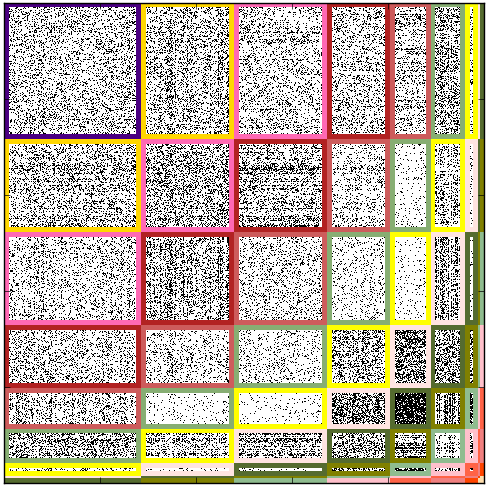
\includegraphics[width=2.94cm, height=3cm]{img/M_g_peaks/figure_6}
	\endminipage
		\minipage{0.17\textwidth}
	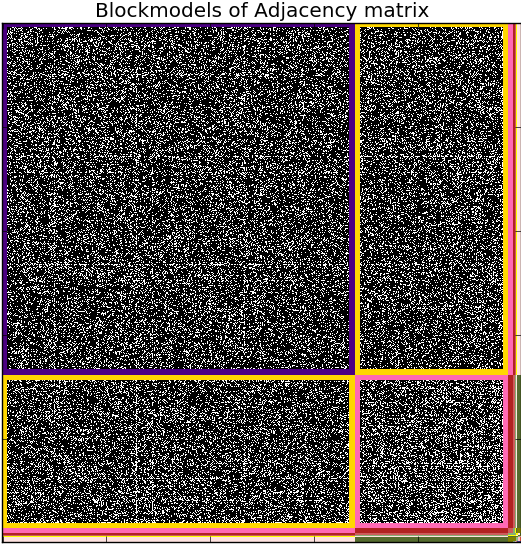
\includegraphics[width=2.94cm, height=3cm]{img/M_g_power_law/figure_6}
	\endminipage
	\minipage{0.17\textwidth}
	\includegraphics[width=2.94cm, height=3cm]{img/M_g_regular/figure_6}
	\endminipage
	%\vspace{-0.3cm}
    \vspace{0.3cm}
	\minipage{0.16\textwidth}
	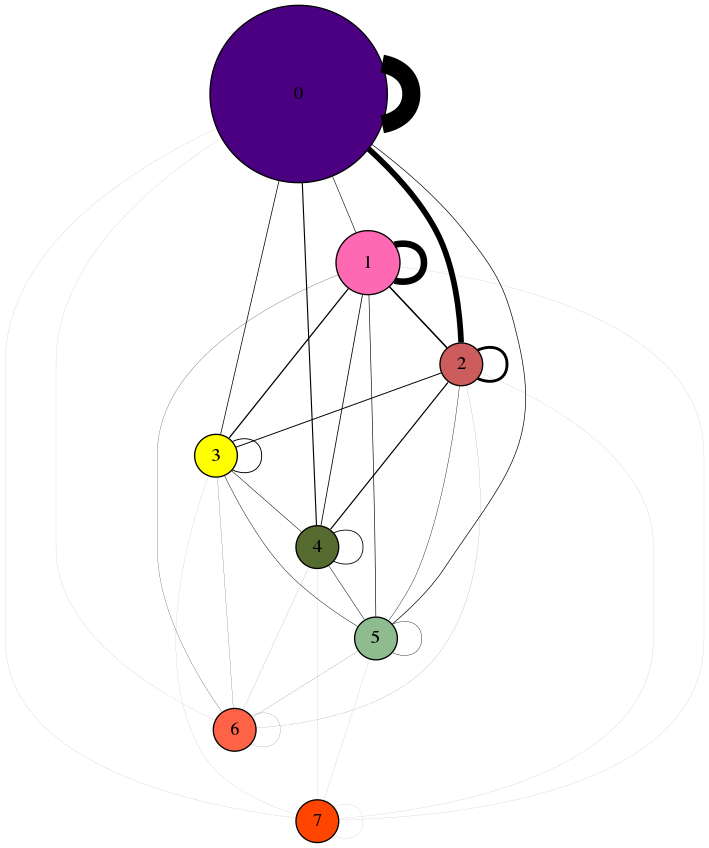
\includegraphics[width=3.5cm, height=4cm]{img/M_g_peaks/graph_dot}
	\endminipage
		\minipage{0.16\textwidth}
    \hspace{1cm}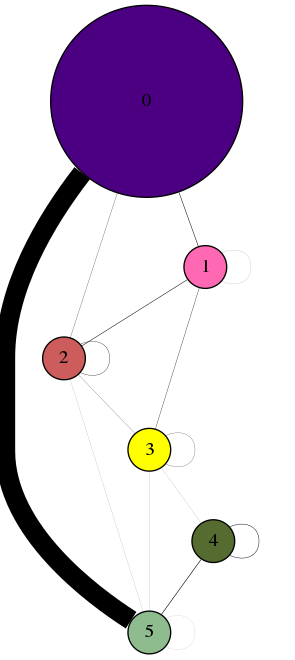
\includegraphics[width=3.0cm, height=4cm]{img/M_g_power_law/graph_dot} 
	\endminipage
	\minipage{0.16\textwidth}
	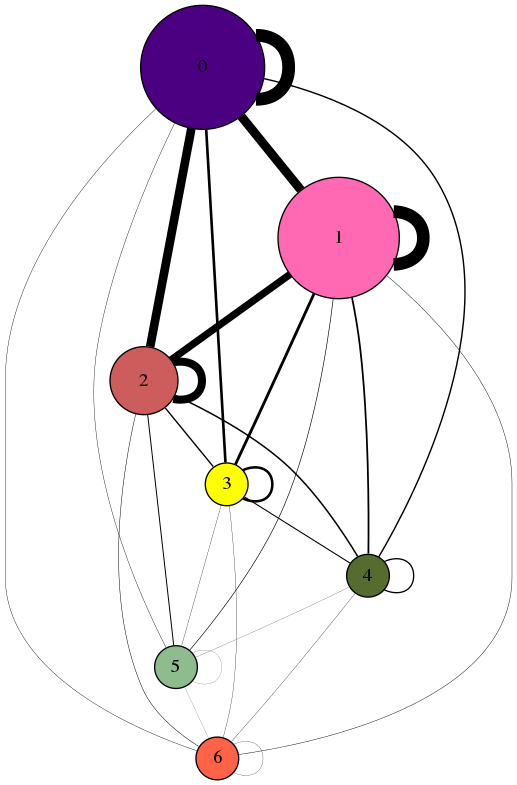
\includegraphics[width=3.5cm, height=4cm]{img/M_g_regular/graph_dot}
	\endminipage
	\caption{Block structure for IMMSB for 3 generated networks. The 3 columns represent 3 different settings. The first row represent the block structure draw on the adjacency matrix. The second row represent the graph of the underlying block structure.}
	\label{fig:gen_blocks_mmsb}
\end{figure}


 We now turn to the burstiness effect.

\section{Burstiness}
\emph{The rich get richer and the poor get poorer} ~\\

%\paragraph{Formal Definition}~\\

The preferential attachment states that a node is more likely to create connections with nodes having a high degree. To take into account this behavior, in the BarabasiAlbert (BA) model, each node is connected to an existing node with a probability proportional to the number of links of the chosen node. This leads to scale-free networks, characterized by a degree distribution with a heavy tail which can be approximated by a power law distribution such that the fraction of nodes $\pr(d)$ having a degree $d$ follows $\pr(d) \sim d^{-\gamma}$ where $\gamma$ ranges typically between 2 and 3~\cite{barabasi1999emergence}. An equivalent notion is the burstiness, studied by~\cite{church1995poisson}, which conveys the same idea : rich get richer or the more you have, the more you will get. In~\cite{clinchant2008bnb}, a formalized definition has been proposed. According to the authors:

\begin{definition}[Burstiness]
	A discrete distribution $\pr$ is bursty if and only if for all integers $(n, n')$, $n \geq n'$ :
	\begin{equation}
	\pr(d \geq n'+1 \mid d \geq n') > \pr(d \geq n+1 \mid d \geq n) 
	\end{equation}
	 A distribution which verifies this condition is said to be bursty.
\end{definition}

In~\cite{clinchant2010information}, this definition has been generalized to the continuous case but, in the sequel, we will retain this first definition since we focus on discrete distributions.~\\

The burstiness can appear for different various variable in a model. In this paper we consider three different schemes at the node and feature level, that constitute some basic assumptions on networks:

\begin{proposition}~\\
for all $i,j \in V^2$ and $k \in \{1,.., K\}$, we have:
\begin{itemize}
	\item Preferential Attachment: the distribution of degree $d_i$ is bursty iff $f_i$ is a stricly increasing function of n with: $$f_i(n)=\pr(y_{ij}=1 \mid d_i=n)$$
	\item Local Preferential Attachment: Given a class couple $c= \{k, k'\} \in \{1,..,K\}^2$, and a degree restricted to nodes who belongs to this interaction couple $d_{ic}$, the distribution of degree $d_{ic}$ is bursty iff $f_{i,c}$ is a stricly increasing function of n with: $$f_{i,c}(n)=\pr(y_{ij}=1 \mid d_i=n, c)$$
	\item Feature burstiness (block/class burstiness ?:s): the distribution over the number of membership of each class is bursty iff  $f_k$  is a stricly increasing function of n with: $$f_k(n) = \pr(\theta_{ik} \mid \theta_{\bm{.}k}^{-ik}=n)$$ 
\end{itemize}
\end{proposition}

We justify this approach in the supplementary materials~\ref{burst_proof}. One can see that the approach makes the link with the classical definition of preferential attachment. Furthermore one can see that the similaraty between th functions we track $(f_i, f_{i,c}, f_k)$ and the typical Gibbs updates. The difference is that we want to assess the generative model given the data and parameters of the model (ie the model has converged). Hence we are looking if the topological property of burstiness can be handle by the model once it learned from the data.~\\


%Considering the nodes projection on latent variables, the projections for the nodes we evaluate might be considered either known or not known ($\Theta$ or $\Theta^{-ij}$) depending on the case study of preferential attachment or local preferential attachment.~\\

\subsection{Burstiness for ILFM}

In this model, the weight interaction matrix $\Phi$ are not conjugate of the likelihood. Thus it can not be integrated out into a closed form expression. As a matter of simplicity we consider this parameter as known, and omit it the following conditional distributions.

Let $F=\Theta$ and $W=\Phi$, each node $i$ has a fixed feature vector noted $F_i$ and a weighed interactions matrix $W$. In this case, the function $f_i$ is:
\begin{align}
&\pr(y_{ij}=1 \mid d_i, F^{-i\bm{.}}) = \sum_{F_i} \pr(y_{ij}=1 \mid d_i, F^{-i\bm{.}} F_i,) \pr(F_i \mid d_i, F^{-i\bm{.}}) \\
&= \sum_{F_i} \sigma(F_iWF_j^T) \frac{\pr(d_i \mid F^{-i\bm{.}}, F_i) \pr(F_i\mid F^{-i\bm{.}}) }{\pr(d_i\mid F^{-i\bm{.}})}\\
&\propto \sum_{F_i} \prod_{j' \in \V(i) \cup {j}} \sigma(F_iWF_{j'}^T)\prod_{j' \notin \V(i)} 1-\sigma(F_iWF_{j'}^T) \prod_k \frac{m_{ik}}{N}
\end{align}

The term $\prod_k \frac{m_{ik}}{N}$ latter equation comes from the conditional probability of a feature $f_{ik}$ for an IBP prior and applying a chain of product rule. The product is the only term that depend on $d_i$ and we refer to it as $f(d_i)$.
Under the assumption that all observed links have higher probability than the observed non-links to bind, we can choose an index dictionary $g$ to reorder the terms such as:
\begin{equation}
\underbrace{\sigma(F_iWF_{g(1)}^T) \geq .. \geq\sigma(F_iWF_{g(p)}^T) }_\text{$g(.) \in \V(i) \cup {j}$ }\geq \underbrace{ .. \geq \sigma(F_iWF_{g(N)}^T)}_\text{$g(.) \notin \V(i)$}
\end{equation}
We then have with some regularity:

\begin{align}
&f(d_i)\geq \sigma(F_iWF_{g(p)}^T)^{d_i +1} (1 - sigma(F_iWF_{g(p+1)}^T))^{N - d_i} \\
&log(f(d_i)) \geq d_i log(\frac{\sigma(F_iWF_{g(p)}^T)}{1-  \sigma(F_iWF_{g(p+1)}^T)}) + cst
\end{align}


Reste a valider 2 point:
\begin{itemize}
	\item Le passage à la proportion
	\item Borner $log(f(d_i))$ entre deux fonction croissantes et montrer qu'on oscille pas à l'intérieur ?!
\end{itemize}

Then a sufficient condition for the burstiness is to have: $\sigma(F_iWF_{g(p)}^T) > 1- \sigma(F_iWF_{g(p+1)}^T)$. If $\sigma$ is the sigmoid this is equivalent ot have $F_iWF_{g(p)}^T > - F_iWF_{g(p+1)}^T$. 

In other term to enable burstiness in the ILFM, the model need to ensure some deterministic behavior when regarding the realization of outcomes and there actual distribution.
%The probability that a matrix $F$ is generated from the IBP is ~\cite{IBP}:
%\begin{equation}
%P(F \mid \alpha) = \frac{\alpha^{K_+}}{\prod_{i=1}^N K_1^{(i)} } \exp(-\alpha H_N) \prod_{k=1}^{K_+} \frac{(N - m_k)!(m_k - 1)!}{N!}
%\end{equation}

\subsection{Burstiness for MMSB}

\label{burst_class}

In the latent class models each  dyads has two underlying  class assignments for each node of the couple. We note $Z \in N\times N\times 2$ the matrix that represents those class assignments.
We seek for the following form of the likelihood, that we marginalize over all the possible couples classes $c=(k, k')$:
\begin{equation} \label{eq:q}
\pr(y_{ij}=1 \mid Y^{-i\bm{.}}, Z^{-ij}, d_i ) = \sum_{c=(k, k')} \pr(y_{ij}=1 \mid Y^{-i\bm{.}}, d_i , c) \pr(c \mid  Z^{-ij} ) 
\end{equation}
Here note that within the sum, the left hand term is conditionally independent of $Z^{-ij}$. And the right hand term is independent of the adjacency terms $Y^{-i\bm{.}}$ since it do not belongs to the Markov blanket of $c$ random variable.

The first term is the likelihood for the links between $(i,j)$ given the class of each node (k, k'). Due to the Beta-Bernoulli conjugacy of the model, $\phi$ and $\theta$ can be marginalized out, and it simplify to: 
\begin{equation} \label{eq:qc}
\pr(y_{ij}=1 \mid Y^{-i\bm{.}}, d_i , c) = \frac{C_{c1}^{-i.} + d_{ic} + \lambda_1}{C_{c\bm{.}}^{-ij} + \lambda_0+\lambda_1} 
\end{equation}
Where $C_{c1}$ denotes the count matrix for all interactions having value 1 (link present) with the classes couple being $c=(k, k')$. Thus $C_{c1} = \sum_{i,j} \bm{1}(z_{i\rightarrow j}=k, z_{i\leftarrow j}=k', y_{ij}=1)$ and $C_{c.} = \sum_{i,j} \bm{1}(z_{i\rightarrow j}=k, z_{i\leftarrow j}=k')$\\

We recognize the likelihood form of the Gibbs update~\cite{HDP}, except that we isolate the term depending of the degree on $i$, $d_i$. Hence the term $d_{ic}$ is the element of the degree with a classes couple $c=(k,k')$ and $d_{ic} = \sum_{j' \neq j} \bm{1}(z_{i\rightarrow j'}=k, z_{i\leftarrow j'}=k', y_{ij'}=1) $.\\

The second term of equation \eqref{eq:q}, can be rewrited by noting that the classes of the couple $c$ are independent and that the term $Y^{-j\bm{.}}$ can be dropped because it is not present in the Markov blanket of the class assignment: 
\begin{equation} \label{eq:topic_assign}
\pr(c \mid  Z^{-ij} ) =  \pr(z_{i\rightarrow j}=k \mid Z^{-ij}) \pr(z_{i\leftarrow j}=k' \mid Z^{-ij})
\end{equation}

Again, the two members of the right hand equation \eqref{eq:topic_assign} are the Gibbs updates for the topic assignments of nodes for the interaction $(i,j)$. Both members reduce to simple form due to the conjugacy between the Dirichlet and Multinomial~\cite{DM} or concurrently from the Chinese Restaurant Franchise~\cite{HDP}:
\begin{align}
\pr(z_{i\rightarrow j}=k \mid Z^{-ij}) = \frac{N_{ik}^{-ij} + \alpha_k}{ N_{i.}^{-ij} + \alpha_{\bm{.}} } \\
\pr(z_{i\leftarrow j}=k' \mid Z^{-ij}) = \frac{N_{jk'}^{-ij} + \alpha_{k'}}{ N_{j\bm{.}}^{-ij} + \alpha_{\bm{.}} } 
\end{align}

Finally, one can see that the only term depending on the degree $d_i$ is isolated, and we can rewrite equation \eqref{eq:q}, with term depending only on $d_i$, $k$, $i$ and $j$:
\begin{equation}
\pr(y_{ij}=1 \mid Y^{-i\bm{.}}, Z^{-ij}, d_i ) = \sum_{c=(k, k')} A_c (B_c + d_{ic})
\end{equation}
Where $A_c$ and $B_c$ are two positive function of $c$.
\begin{align}
A_c &= \frac{N_{ik}^{-ij} + \alpha_k}{ N_{i.}^{-ij} + \alpha_{\bm{.}} } \frac{N_{jk'}^{-ij} + \alpha_{k'}}{ N_{j\bm{.}}^{-ij} + \alpha_{\bm{.}} } \frac{1}{C_{c\bm{.}}^{-ij} + \lambda_0+\lambda_1} \\
B_c &= C_{c1}^{-i.} + \lambda_1
\end{align}

As we sum over all possible couple classes, the probability to have a link will augment with the degree with the classes couple corresponding to the element of the degree with the same couple. Hence the probability to observe a link for node $i$ is strictly crescent with his degree $d_i$. 

\paragraph{Preferential Attachment}~\\

The model is bursty hence it can handle the preferential attachment at the network level.

\paragraph{Local Preferential Attachment}~\\

The Local preferential attachment is similar to the notion of burstiness but inside a community/class of the network. Assuming that we know the class of $i$ $z_{i\rightarrow j}$ to be $k$, the probability to have a link becomes: 
\begin{align}
&\pr(y_{ij}=1 \mid Y^{-i\bm{.}}, d_i,z_{i\rightarrow j})  = \sum_{k'} \pr(y_{ij}=1 \mid Y^{-i\bm{.}}, Z^{-ij}, d_i , c=(k,k')) \pr(z_{i\leftarrow j}=k' \mid Z^{-ij} ) \\
&= \sum_{k'} \frac{C_{c1}^{-i.} + d_{ic} + \lambda_1}{C_{c\bm{.}}^{-ij} + \lambda_0 + \lambda_1} \frac{N_{jk'}^{-ij} + \alpha_{k'}}{ N_{j\bm{.}}^{-ij} + \alpha_{\bm{.}} } \\
&= \sum_{k'} A'_{k'} (B'_{k'} + d_{i(k,k')})
\end{align}

Here the probability increases with the degree independently of the interactions classes. This means that burstiness is possible inside but also between communities.

\paragraph{Communities Distribution}~\\

....Need to count the table for each classes in Chinese Restaurant Franchise (CRF), to evaluate the distribution according to the hyperprior of HDP...




\section{Prediction Evaluation}
\label{sec:experiments}

In previous sections, we shown theoretical results with empirical measures  on realization of networks using the generative property of the probabilistic models. In this section, we seek to explain the predictive performance on several datasets by examining their empirical properties and how well the models can capture them. This analysis provide also a study on a comparison of both models, IMMSB and ILFM. Particularly we will see that performance of those models really depend on the type of data we want to fit.

This section is organized as follows:  In first subsection we described our goodness of fit measure used to evaluate various degree distribution. In the second we present the synthetic and real dataset that we have used. In the third we present our prediction evaluation setting. In the last we report our results.

\subsection{A measures for the preferential attachment effect}

\label{sec:experiments-burst}
Preferential attachment leads to networks characterized by a degree distribution with heavy tail. A typical form of such law, often meet in data, is a a power law distribution. Comparison of the degree distribution with a linear function in the log-log scale  gives us a qualitative measure for the preferential attachment. However, for a better evaluation of the power law hypothesis on the degree distribution, we rely on a  goodness a fit based on a Kolmogorov-Smirnov (KS) test. We follow the protocol described in \cite{clauset2009power} which consists of the following steps:
\begin{itemize}
	\item Estimate the parameters $x_{min}$ and $\alpha$ of the power law model.
	\item Calculate the goodness of fit between synthetic datasets generated with the power law and the data. The resulting $p$-values gives an estimates of the  plausibility of the hypothesis for the data.
\end{itemize}

As mentioned in \cite{clauset2009power} high value of the $p$-value should be considered with caution for at least two reasons. First, there may be other distribution that match the data equally or better. Second, a small number of samples of the data may lead to high p-value and reflect the fact that is hard to rule out an hypothesis in such a case.

\subsection{Datasets}
In our experiments, we consider four artificial networks and two real networks.\\

\textit{Artificial networks}

The artificial networks have been generated with ANC-Generator \cite{largeron2015}. This generator has been chosen because it allows to build attributed graphs with  community structure faithfully following the known properties of real-world networks such as preferential attachment and homophily.
Moreover, by modifying the parameters, these properties can be weakened. Finally, ANC-Generator is available under the terms of the GNU Public License and the        parameters can be shared for experiments reproducibility.

Four artificial networks have been generated, each one corresponding to a configuration  regarding the properties of interest.
Table \ref{table:artificial_networks} summarizes these four configurations. We report the seed and parameters that we use those synthetic networks in appendix \ref{seed_dancer	}. Each generated networks correspond to a different combination where homophily and preferential attachment are more or less characterizing the underlying networks. For example...

\begin{table}[h] \label{table:artificial_networks}
	\caption{Artificial networks characteristic.}
	\begin{tabular}{lrrrr}
		\hline
		Networks   &  p-value    &  Modularity & Clustering coefff & density   \\
		\hline
		$Network1$    & 1 &0.59  & 0.06 & 0.007  \\
		$Network2$   & 1 &0.43  & 0.08 & 0.006\\
		$Network3$  & 0.52  &0.71  & 0.49 & 0.01 \\
		$Network4$   & 0.57  &0.68  & 0.61 & 0.06 \\
		\hline
	\end{tabular}
	\caption{Real networks characteristic}
	\begin{tabular}{lrrrr}
		\hline
		Networks    &  p-value    &  Modularity & Clustering coefff & density   \\
		\hline
		$fb\_uc$          & 1 & -  & 0.10 & 0.008 \\
		$manufacturing$   & 0.42 & -  & 0.59 & 0.24 \\
	\end{tabular}
\end{table}

\textit{Real networks}

We also used two real world networks for our experiments .
The first one \footnote{available at:} is built from an online community of 1899 students from the University of California. Each node corresponds to a user and a    directed edge represents a sent message.
The second one \footnote{available at:} is an internal email communication network between employees of a mid-sized manufacturing company. Each vertex is associated  to an employee and an oriented link represents like previously a sent email.

Table 1 summarizes some properties characteristics of these artificial and real datasets. The  p-value is computed as described in \ref{sec:experiments-burst } as a reference for the global preferential attachment effect. we also report the modularity on the a given (true) partition (by Dancer) of the networks, and the clustering coefficient.

\begin{figure}[h]
	\centering
	
	\minipage{0.25\textwidth}
	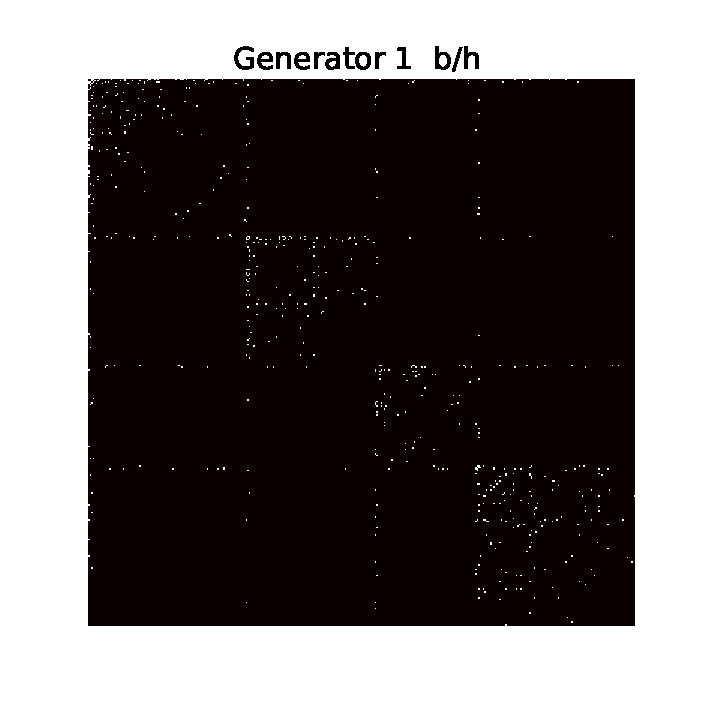
\includegraphics[scale=0.4]{\lpath/img/g1}
	\endminipage
	\minipage{0.25\textwidth}
	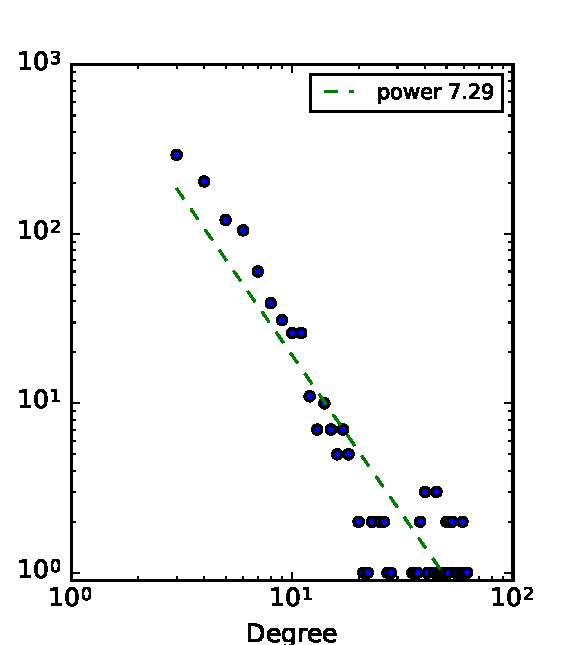
\includegraphics[scale=0.4]{\lpath/img/g1_d}
	\endminipage
	\vspace{-0.4cm}
	\minipage{0.25\textwidth}
	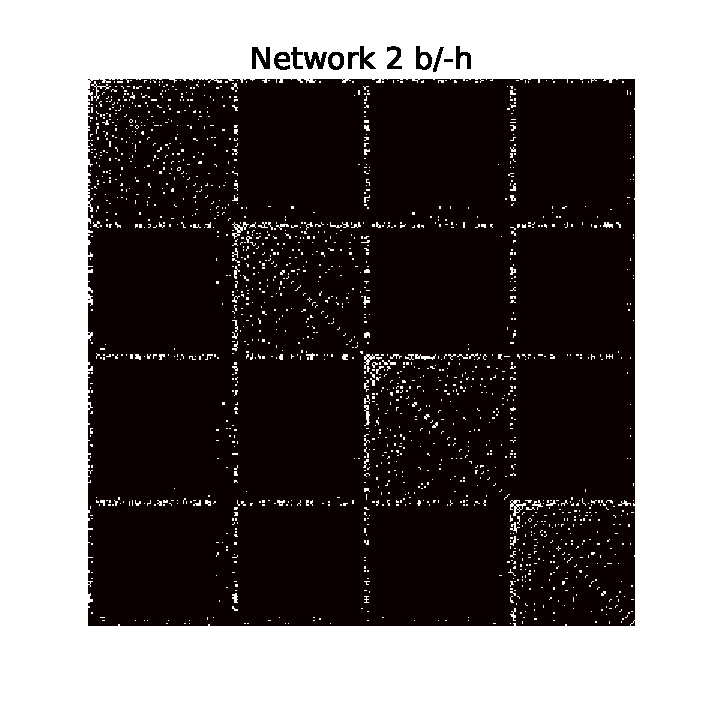
\includegraphics[scale=0.4]{\lpath/img/g2}
	\endminipage
	\minipage{0.25\textwidth}
	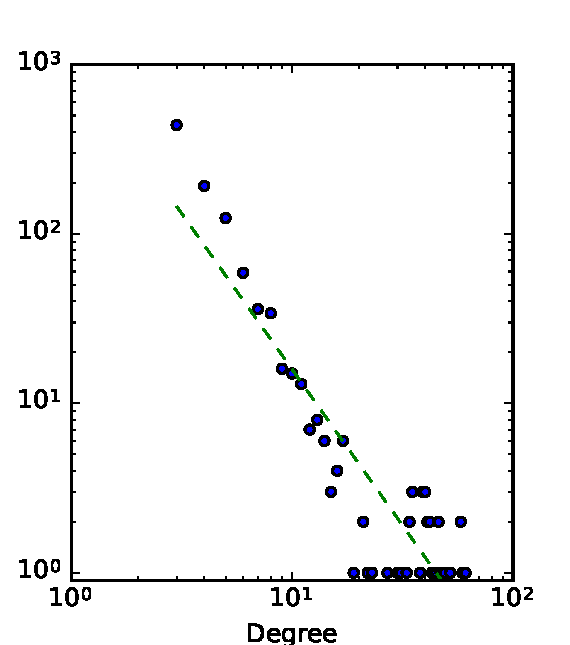
\includegraphics[scale=0.4]{\lpath/img/g2_d}
	\endminipage
	\vspace{-0.4cm}
	\minipage{0.25\textwidth}
	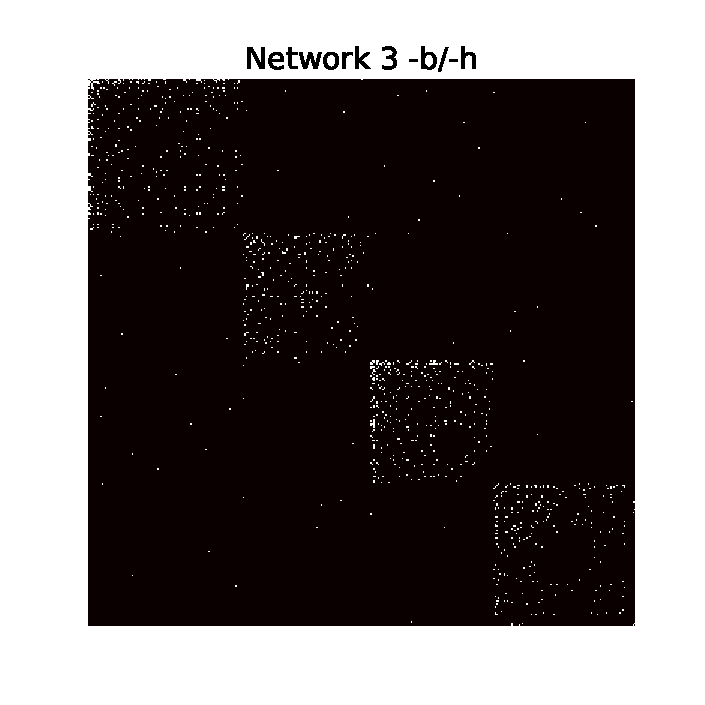
\includegraphics[scale=0.4]{\lpath/img/g3}
	\endminipage
	\minipage{0.25\textwidth}
	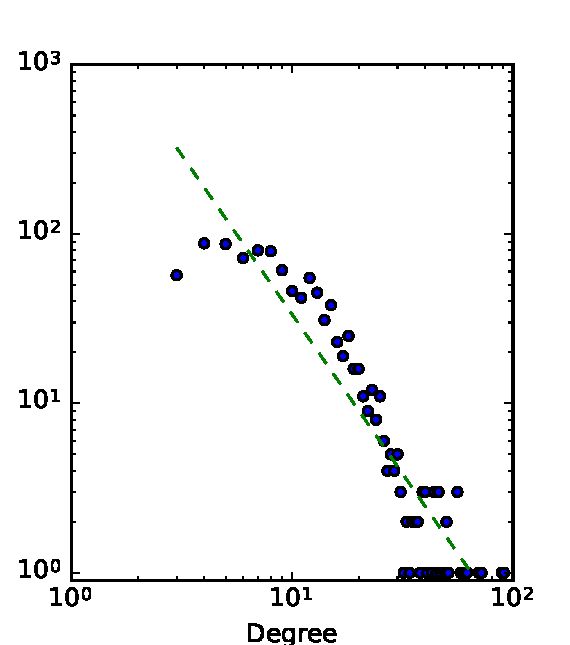
\includegraphics[scale=0.4]{\lpath/img/g3_d}
	\endminipage
	\vspace{-0.4cm}
	\minipage{0.25\textwidth}
	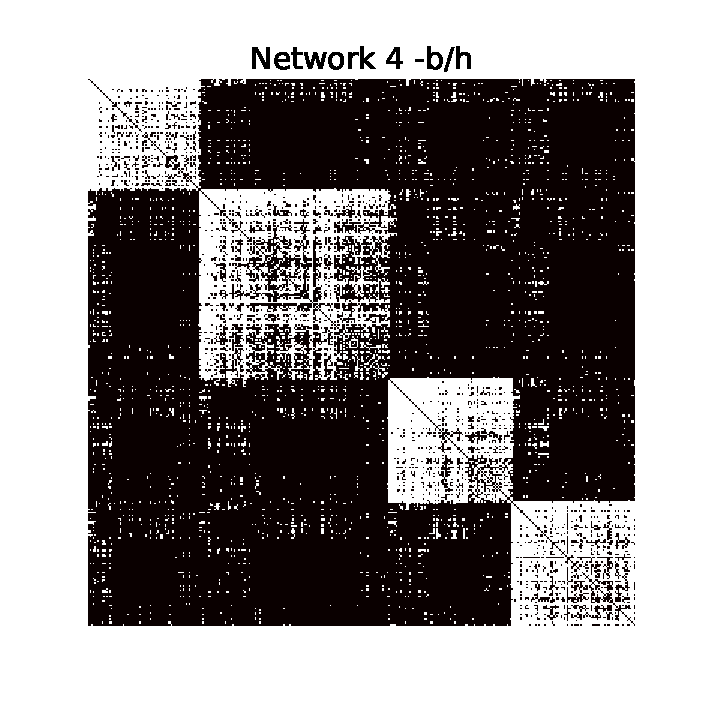
\includegraphics[scale=0.4]{\lpath/img/g4}
	\endminipage
	\minipage{0.25\textwidth}
	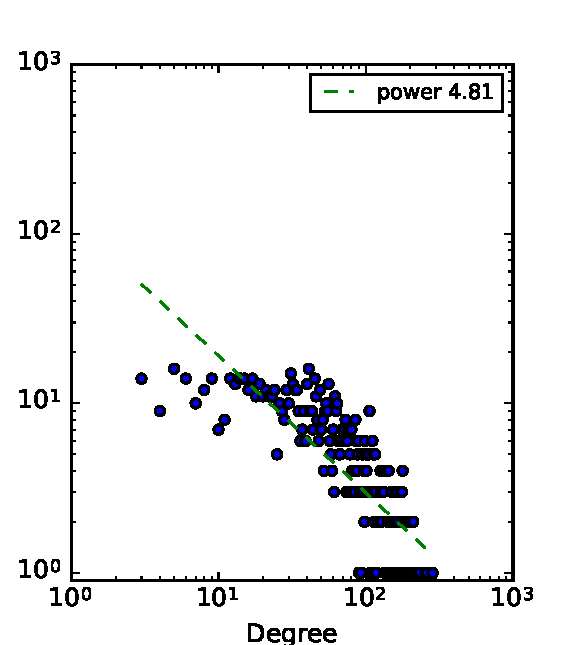
\includegraphics[scale=0.4]{\lpath/img/g4_d}
	\endminipage
	
	\caption{Left figures represent the adjacency matrices (left) for each of the 4 synthetic networks that we used for the prediction evaluation along their respective global degree distribution in the right plots.}
	\label{fig:synt_graph}
\end{figure}

\begin{figure}[h]
	\centering
	
	
	\minipage{0.25\textwidth}
	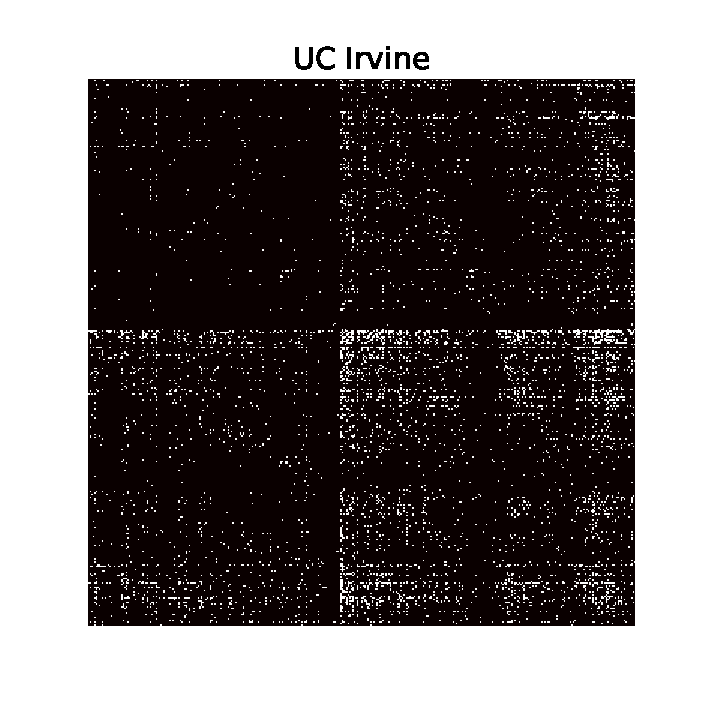
\includegraphics[scale=0.4]{\lpath/img/irvine}
	\endminipage
	\minipage{0.25\textwidth}
	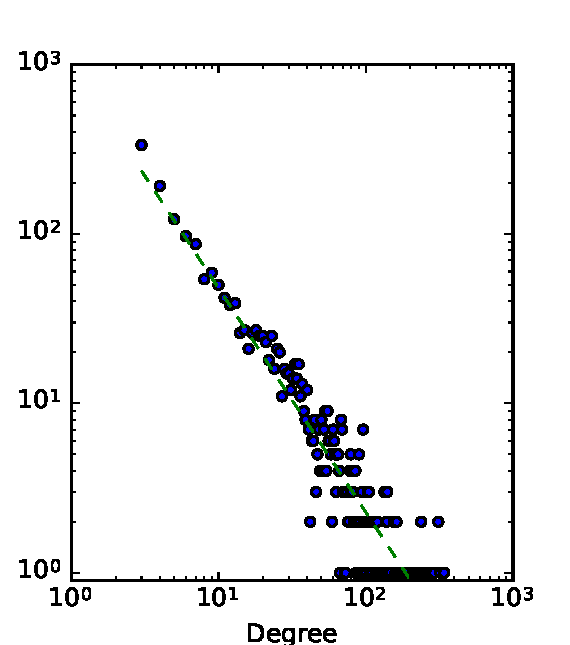
\includegraphics[scale=0.4]{\lpath/img/irvine_d}
	\endminipage
	\vspace{-0.4cm}
	\minipage{0.25\textwidth}
	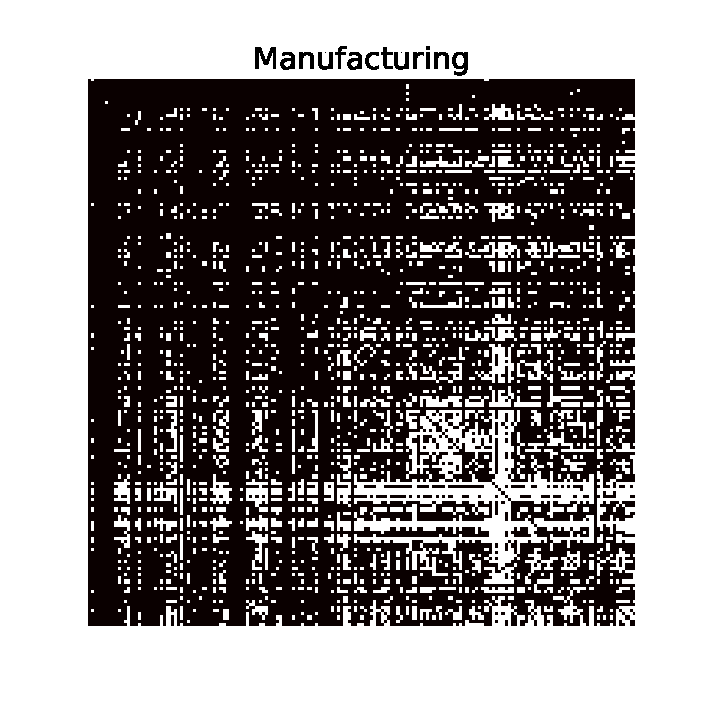
\includegraphics[scale=0.4]{\lpath/img/manufacturing}
	\endminipage
	\minipage{0.25\textwidth}
	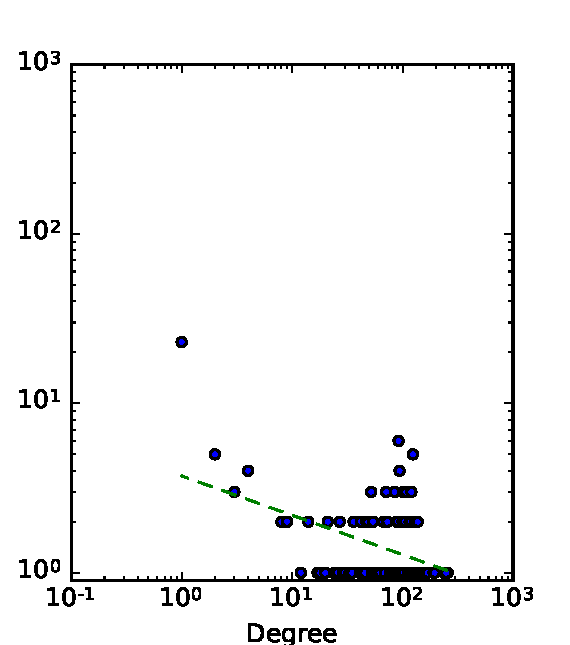
\includegraphics[scale=0.4]{\lpath/img/manufacturing_d}
	\endminipage
	\caption{Left figures represent the adjacency matrices (left) for each of the 2 real networks that we used for the prediction evaluation along their respective global degree distribution in the right plots.}
	\label{fig:real_graph}
\end{figure}



\subsection{Experimental Settings}
For each datasets described,  we run a MCMC inference consisting of 200 iterations to learn the posterior distribution of each the IMMSB model and ILFM, described in \ref{sec:models}. For IMMSB, concentration parameters of HDP were optimized following \cite{HDP} using vague gamma priors $\alpha_0 \sim \text{Gamma}(1,1)$ and       $\gamma \sim \text{Gamma}(1,1)$. The parameter for the matrix weights were fixed to $\lambda_0=\lambda_1=0.1$. For ILFM, the IBP hyper-parameter was fixed to   $\alpha=0.5$ and the weights hyper-parameter to $\sigma_w = 1$. Each experiences were averaged on 10 repetitions, and results were found to be stable regarding on the random  initialization and the stochastic optimization procedure. 
 

We evaluate the  prediction performance of the models by building a training set and a testing set from the original datasets. In order to achieve this, we build a random mask consisting of 20 percent of the size of the adjacency matrix. This mask is used a our testing set, while the 80 remaining percent are used as a training set.

The inference procedure was run under this settings in all of the 4 synthetic datasets and 2 real networks.

All our experimental platform is available online \footnote{https://github.com/dtrckd/pymake}. It is an ongoing development in order to provide a flexible way to design and run experiments and make data analysis.


\begin{figure}[h]
	\centering
	
	\minipage{0.25\textwidth}
	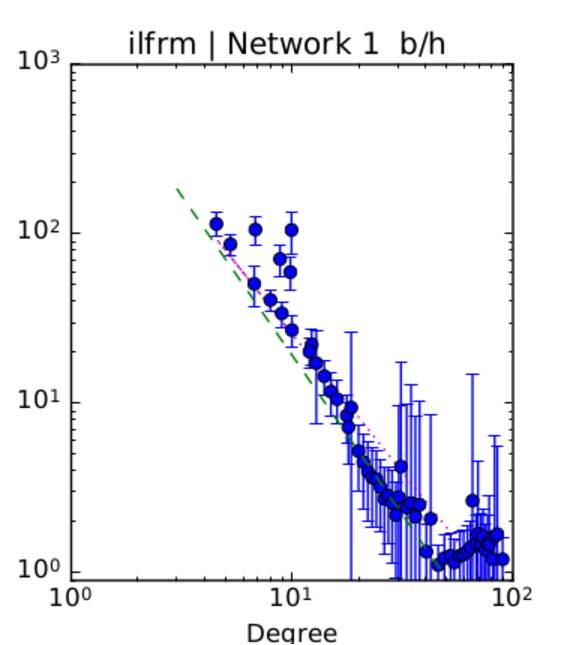
\includegraphics[scale=0.4]{\lpath/img/ilfrm_g1_d}
	\endminipage
	\minipage{0.25\textwidth}
	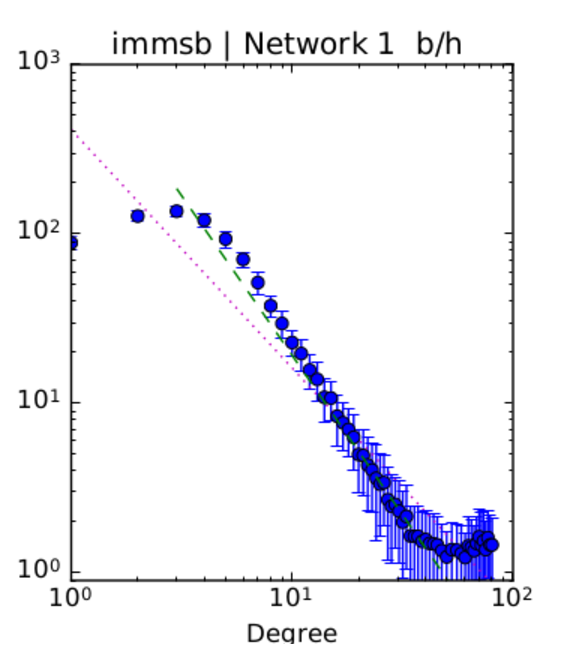
\includegraphics[scale=0.4]{\lpath/img/immsb_g1_d}
	\endminipage
	\vspace{-0.4cm}
	\minipage{0.25\textwidth}
	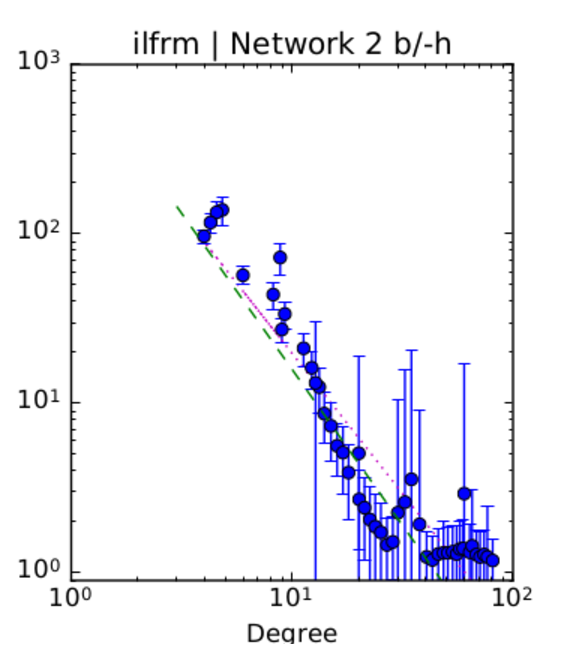
\includegraphics[scale=0.4]{\lpath/img/ilfrm_g2_d}
	\endminipage
	\minipage{0.25\textwidth}
	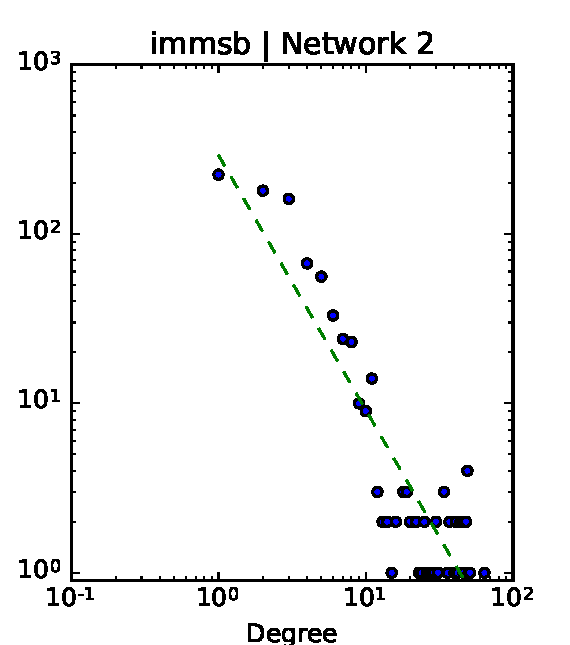
\includegraphics[scale=0.4]{\lpath/img/immsb_g2_d}
	\endminipage
	\vspace{-0.4cm}
	\minipage{0.25\textwidth}
	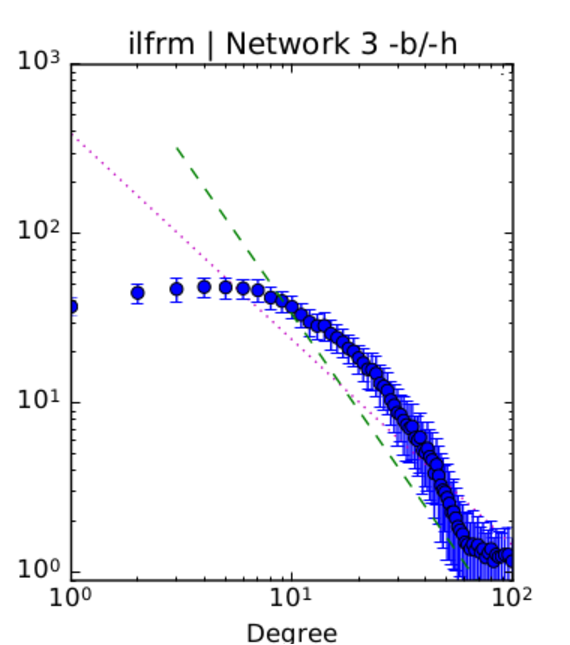
\includegraphics[scale=0.4]{\lpath/img/ilfrm_g3_d}
	\endminipage
	\minipage{0.25\textwidth}
	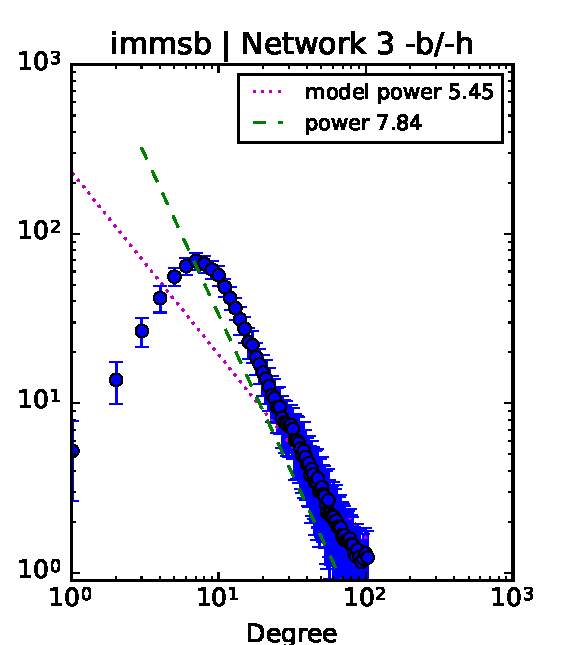
\includegraphics[scale=0.4]{\lpath/img/immsb_g3_d}
	\endminipage
	\vspace{-0.4cm}
	\minipage{0.25\textwidth}
	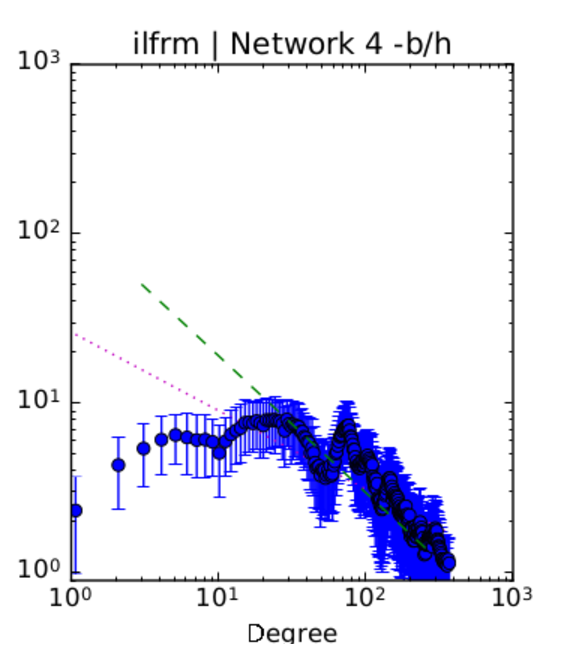
\includegraphics[scale=0.4]{\lpath/img/ilfrm_g4_d}
	\endminipage
	\minipage{0.25\textwidth}
	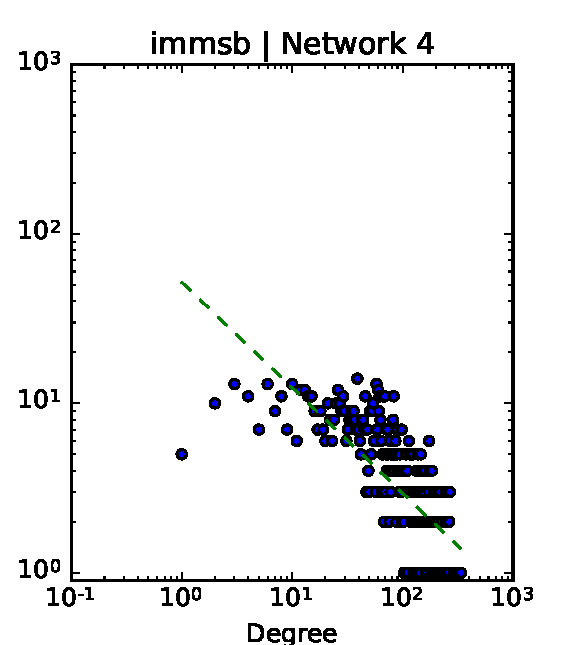
\includegraphics[scale=0.4]{\lpath/img/immsb_g4_d}
	\endminipage
	
	\caption{Right column is associated to IMMSB and left column to ILFM. Each row is associated to a synthetic networks on which we run the inference procedure. Each figures represent the global degrees distribution for a set of 100 generated networks by the models after its parameters where learned in the corresponding settings.  We also report on these figures two straight lines corresponding of the regression on the degree distribution of the model generated network (dotted) and the regression of the original distribution (dashed) as a qualitative reference.}
	\label{fig:gen_graph_s}
\end{figure}

\begin{figure}[h]
	\centering
	
	\minipage{0.25\textwidth}
	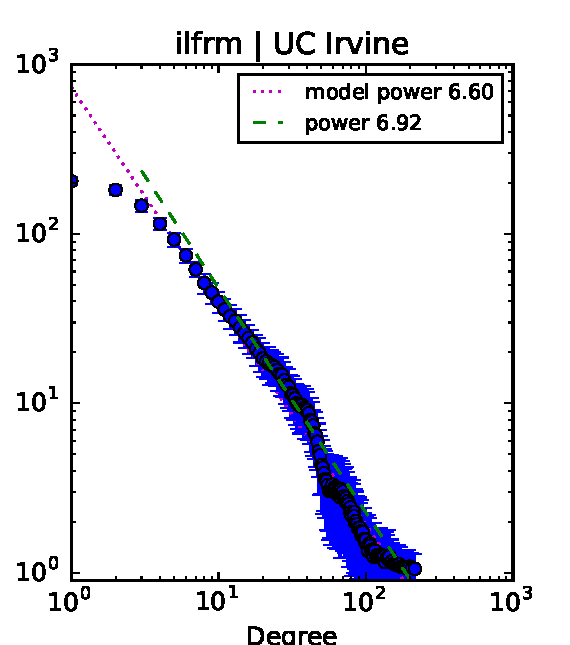
\includegraphics[scale=0.4]{\lpath/img/ilfrm_irvine_d}
	\endminipage
	\minipage{0.25\textwidth}
	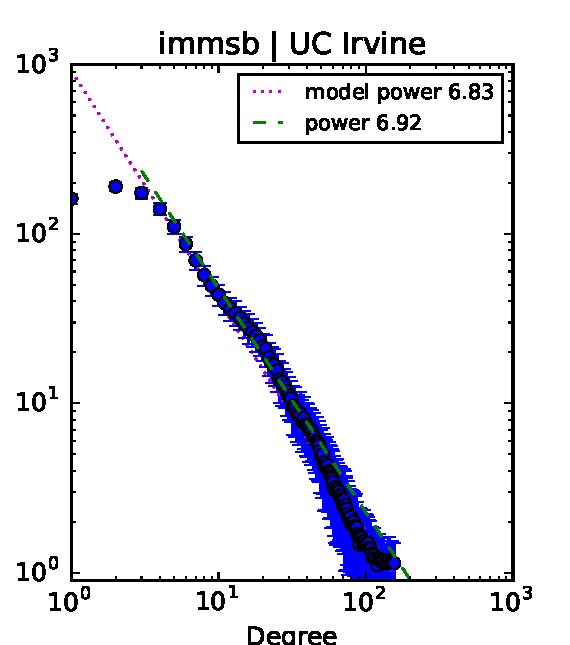
\includegraphics[scale=0.4]{\lpath/img/immsb_irvine_d}
	\endminipage
	\vspace{-0.4cm}
	\minipage{0.25\textwidth}
	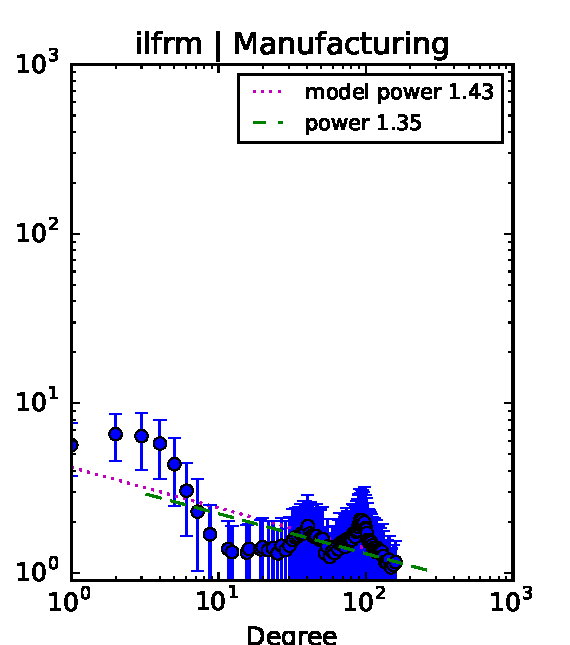
\includegraphics[scale=0.4]{\lpath/img/ilfrm_manufacturing_d}
	\endminipage
	\minipage{0.25\textwidth}
	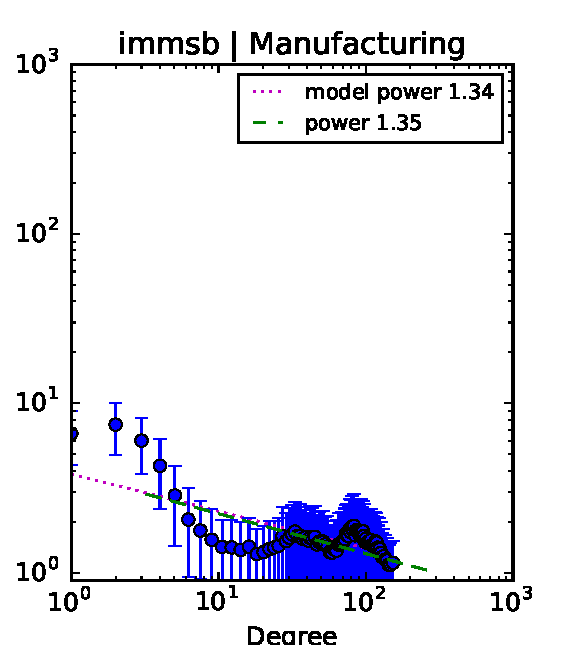
\includegraphics[scale=0.4]{\lpath/img/immsb_manufacturing_d}
	\endminipage
	
	\caption{Right column is associated to IMMSB and left column to ILFM. Each row is associated to a real networks on which we run the inference procedure. Each figures represent the global degrees distribution for a set of 100 generated networks by the models after its parameters where learned in the corresponding settings. We also report on these figures two straight lines corresponding of the regression on the degree distribution of the model generated network (dotted) and the regression of the original distribution (dashed) as qualitative reference.}
	\label{fig:gen_graph_r}
\end{figure}


\begin{figure}[h]
	\centering
	
	\minipage{0.25\textwidth}
	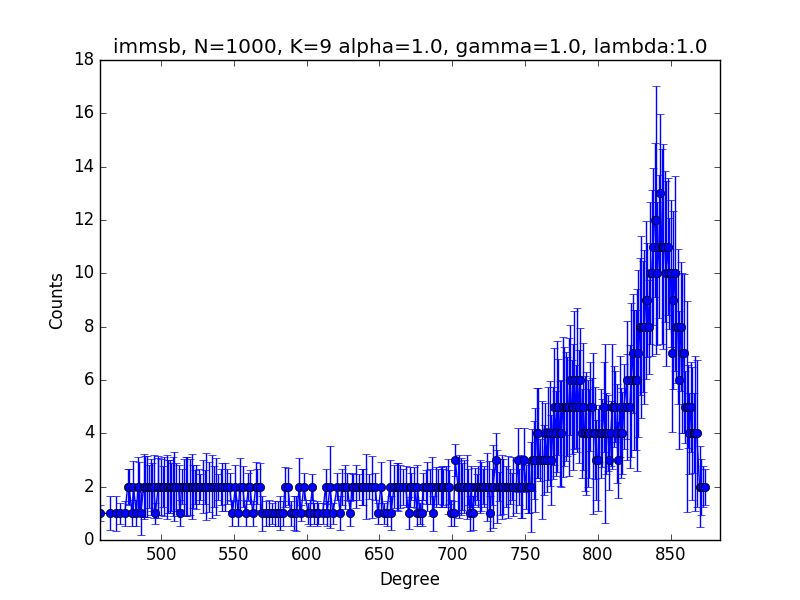
\includegraphics[scale=0.22]{\lpath/img/M_e/AUC-ROC/figure_1}
	\endminipage
	\minipage{0.25\textwidth}
	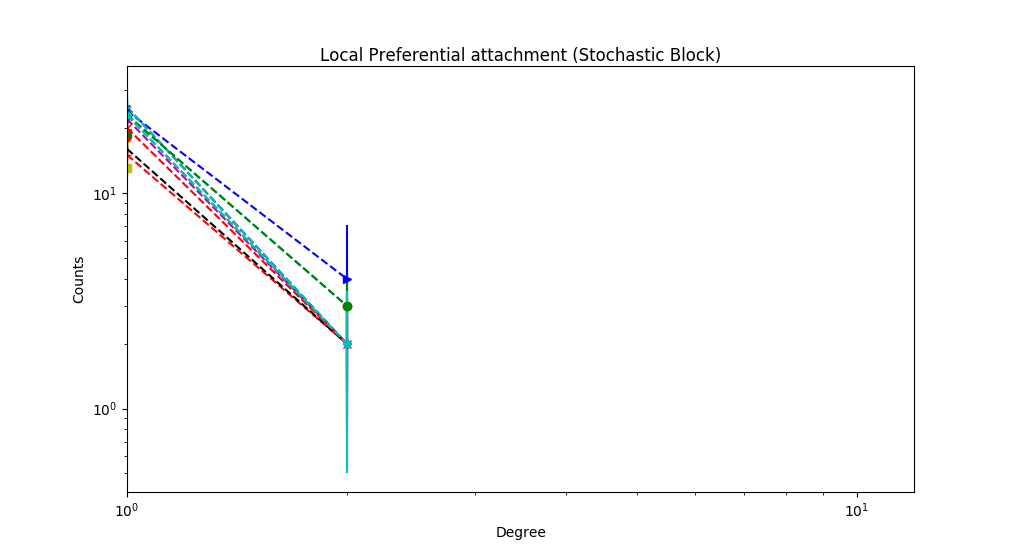
\includegraphics[scale=0.22]{\lpath/img/M_e/AUC-ROC/figure_2}
	\endminipage
	\vspace{-0.4cm}
	\minipage{0.25\textwidth}
	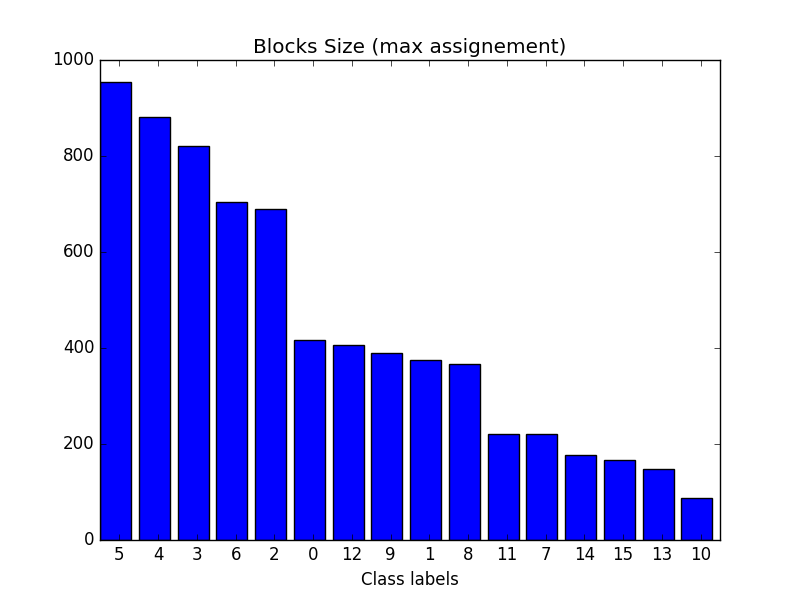
\includegraphics[scale=0.22]{\lpath/img/M_e/AUC-ROC/figure_3}
	\endminipage
	\minipage{0.25\textwidth}
	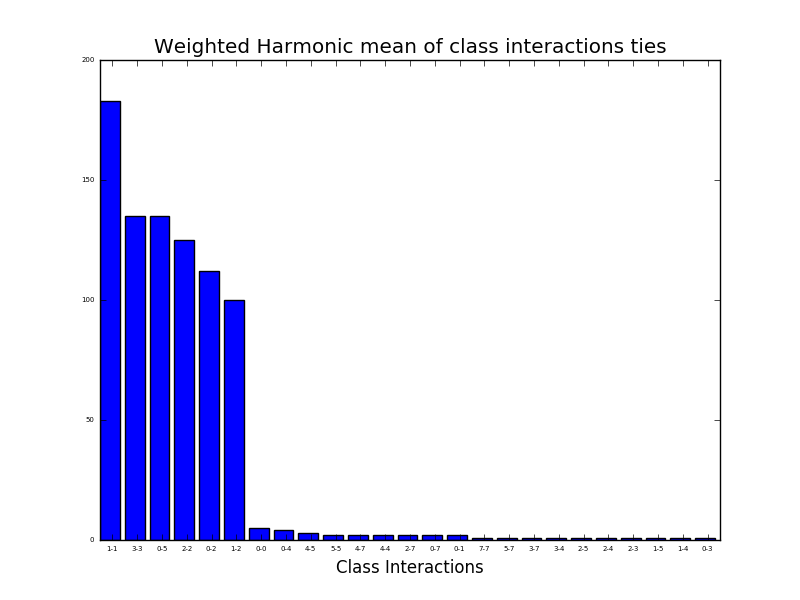
\includegraphics[scale=0.22]{\lpath/img/M_e/AUC-ROC/figure_4}
	\endminipage
		\vspace{-0.4cm}
	\minipage{0.25\textwidth}
	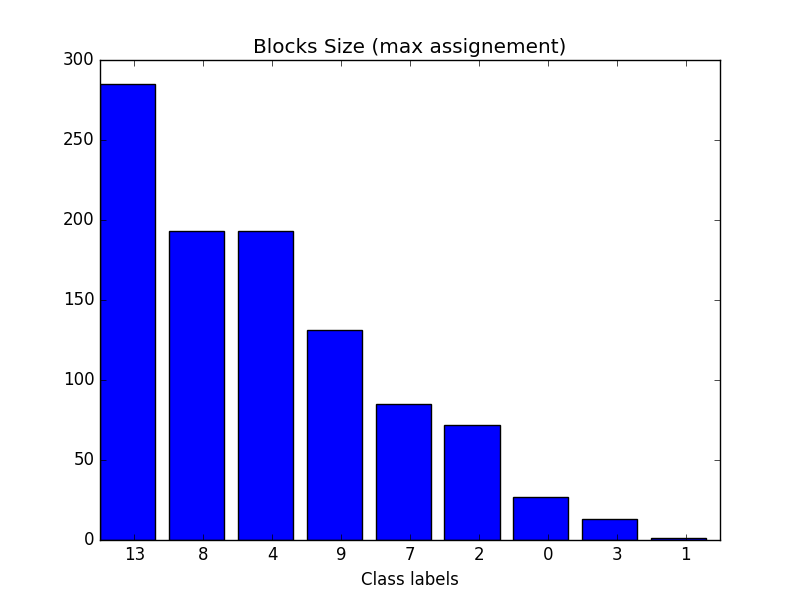
\includegraphics[scale=0.22]{\lpath/img/M_e/AUC-ROC/figure_5}
	\endminipage
	\minipage{0.25\textwidth}
	\includegraphics[scale=0.22]{\lpath/img/M_e/AUC-ROC/figure_6}
	\endminipage
	
	\caption{AUC curves that compare the performance of ILFM and IMMSB on the 4 synthetic networks.}
	\label{fig:auc}
\end{figure}



\subsection{Results}

%%% Figure description:
We report in table \ref{table:unbalanced} our results for the prediction performance in the different settings. The prediction problem is equivalent to a binary prediction problem, where the prediction lies in two classes; edge or not an edge. The local precision and recall in the table concern the links predicted as an edge. The global (precision) refer to the accuracy of the model. The table summarize the precision and recall into the $f_1$ measure. Note that each group of row is indexed by  a number $K$ which indicates various values of initialization of the latent feature dimension.

Comparatively, in figure \ref{fig:auc}, we report the Area Under Curve for each datasets where we compare the prediction performance of IMMSB and ILFM on the task of links prediction.

In figure \ref{fig:gen_graph_s} and \ref{fig:gen_graph_r} we used the models learned on the training datasets to generate full networks and report the global degree distribution of such generated networks. 

%%% What the figure tells:
comparing the performance between both models in the links prediction precision and recall and $F_1$ measure (ref{table:unbalanced}), can seem to conflict with results in the ROC curve (\ref{fig:auc}). More precisely we see that ILFM dominate IMMSB on the $f_1$ measures on all experiments except for one (network 1, K=15). But on the AUC-ROC analysis( \ref{fig:auc}) we see that IMMSB dominate ILFM for two networks (Networks 1 and Networks 2), although it's number of latent feature is almost half lesser than for ILFM. This behavior is also reflected on the accuracy for both models (global precision); The accuracy of IMMSB models is higher for the Network1 and Network2, and this is the opposite for ILFM, which are more accurate for Network3 and Network4. Interestingly, we see that for ILFM, the dimension of the latent feature for which ILFM converged, for the two first networks is significantly higher than the two other. In other words the ILFM model seems to compensate is weak performance by increasing the number of features.

In the other hands, according to the degree distribution of the 4 synthetic networks we fitted, (figure \ref{fig:synt_graph}) and the p-value associated the power law hypothesis (table \ref{table:artificial_networks}), we see that the Network1 and Network2 has a stronger preferential attachment effects than Network3 and Network4.


Finally, the difference of behaviors of the models according to the training networks is captured by the randomness of the (generated) degree distributions (figure \ref{fig:gen_graph_s} ). We see that the degree distribution corresponding to the two bursty synthetic network, has  a high variance for ILFM while it is quite smooth for IMMSB.

The success of ILFM on bursty networks reflects the fact ILFM can handle the local preferential attachments and not ILFM. We assume that this symptom for ILFM is due to the hard assignment of it's latent features, where a difference of one feature, in a feature vector, can lead to a big gap in the probability to generate a link. A phenomenon particularly strong for very bursty networks where the long tail makes the distribution of degrees more sensitive to little change.

\textcolor{red}{Nothing about real networks: result are not really interesting except why ILFM variance of degree distribution on bursty networks fb\_uc is smooth ? }

To conclude, these experiments show that a properties based approach can help to choose an appropriate models. Moreover a model that seems to outperforms an other with a particular measure could be non optimal depending on what we want to capture in the data, keeping in mind that one measures is associated, in some way, to one behaviors or property.

\section{Related Work}
= Prop
Burstiness on topic model:
Modeling Word Burstiness Using the Dirichlet Distribution (DCM)
Accounting for Burstiness in Topic Models (DCMLDA)
LDA bursty on topics
Proposal of a-MMSB in : Scalable Inference of Overlapping Communities
with high diagonal only...

to read: Stochastic blockmodels and community structure in networks

= Model
Recent work on MMSB and copula: Copula Mixed-Membership Stochastic Blockmodel with Subgr
oup Correlation



\section{Conclusion}
\label{sec:concl}

%\section{Supplementary materials}

\subsection{Class based derivation}

\paragraph{Likelihood:}~\\

We mention that  the $\phi$ and $\theta$ matrix can be reconstructed with $Z$. From the model, we have the following equalities:
\begin{align}
\pr(y_{ij} \mid \phi_c) &= \phi_c^{y_{ij}}(1-\phi_c)^{1-y_{ij}} \\
\pr(\phi_c \mid \lambda) &= \frac{1}{B(\lambda_1, \lambda_0)} \phi_c^{\lambda_1-1}(1-\phi_c)^{\lambda_0 -1}
\end{align}


Derivation of equation (5.12) of the likelihood:
\begin{align}
&\pr(y_{ij} \mid Y^{-ij}, c) \propto \pr(y_{ij}, Y^{-ij}, c) \\
&= \int_{\phi_c} \pr(y_{ij} \mid \phi_c) \pr(\phi_c \mid \lambda) \prod_{i'j' \neq ij}\pr(y_{i'j'} \mid \phi_c) d\phi_c \\
&\propto \int_{\phi_c} \phi_c^{y_{ij} + C_{c1}^{-ji} + \lambda_1-1}(1-\phi_c)^{ 1-y_{ij} + C_{c0}^{-ji} + \lambda_0 -1} d\phi_c \\
&\propto \frac{\Gamma(y_{ij} + C_{c1}^{-ji} + \lambda_1) \Gamma( 1-y_{ij} + C_{c0}^{-ji} + \lambda_0) }{\Gamma(  1+ C_{c\bm{.}}^{-ji} + \lambda_0 + \lambda_1)}
\end{align}

Considering the case where $y_{ij} =1$, we have :
\begin{equation}
\pr(y_{ij}=1 \mid \phi_c) = \frac{C_{c1}^{-ji} + \lambda_1}{C_{c\bm{.}}^{-ji} + \lambda_0 + \lambda_1}
\end{equation}


\paragraph{Class Assignment:}~\\

We have from the model the following equalities:
\begin{align}
\pr(\theta_i \mid \alpha) &= \frac{\Gamma(\sum_l \alpha)}{\prod_l \Gamma(\alpha)} \prod_l \theta_{il}^{\alpha-1} \\
\pr(z_{i\rightarrow j} &= k \mid \theta_i) = \theta_{ik}
\end{align}

Derivation of equation (5.14) of class assignment:
\begin{align}
&\pr(z_{i\rightarrow j}=k \mid Z^{-ij}) = \pr(z_{i\rightarrow j}=k \mid \{z_{i\rightarrow j_0}\}_{j_0\neq j},\{z_{i\leftarrow j_0}\}_{j_0= 1}^n )\\
&\propto \pr(z_{i\rightarrow j}= k,\{z_{i\rightarrow j_0}\}_{j_0\neq j},\{z_{i\leftarrow j_0}\}_{j_0= 1}^n ) \\
&= \int_{\theta_i} \pr(\theta_i \mid \alpha) \pr(z_{i\rightarrow j}=k \mid \theta_i) \prod_{j_0\neq j} \pr(z_{i\rightarrow j_0} \mid \theta_i) \prod_{j_0 =  1}^n  \pr(z_{i\leftarrow j_0} \mid \theta_i)  d\theta_i \\
&=\int_{\theta_i} \frac{\Gamma(\sum_l \alpha)}{\prod_l \Gamma(\alpha)}\theta_{ik}^{N_{ik}^{-ji}+1} \prod_{l\neq k} \theta_{il}^{N_{il}^{-ij} +\alpha-1} d\theta_i \\
&\propto \frac{\Gamma(\alpha + N_{ik}^{-ji}+1)\prod_{l\neq k} \Gamma(\alpha + N_{il}^{-ij})}{\Gamma(\sum_l( \alpha + N_{il}^{-ji}) +1)} \\
&\propto \alpha + N_{ik}^{-ji}
\end{align}

Finally the equality is maintain by the marginalization constant:
\begin{equation}
\pr(z_{i\rightarrow j}=k \mid Z^{-ij}) =\frac{ N_{ik}^{-ji} + \alpha}{ N_{i\bm{.}}^{-ji} + K\alpha }
\end{equation}

\subsection{Burstiness for degrees Distribution}
\label{burst_proof}

From the definition of the burstiness, we have for a random variable $d$:
\begin{equation}
	\pr(d \geq n'+1 \mid d \geq n') > \pr(d \geq n+1 \mid d \geq n) \quad \{\forall (n,n') \mid  n' > n \}
\end{equation}

We now consider the degree $d_i$ for a node $i$ of a network. We can rewrite the burstiness in the discrete case:
\begin{equation}
\pr(d_i = n'+1 \mid d_i = n') > \pr(d_i = n+1 \mid d_i = n), \quad \{\forall (n,n') \mid  n' > n \}
\end{equation}
\hspace{0.35\textwidth} Q. is it equivalent to: $\pr(d_i)' > 0$ ?\\

Let's suppose that the model $\mathcal{M} = \{\Theta, \Phi\}$ has converged to some local optima. Do new predictions will respect the burstiness property ? To answer this question we need to evaluate the predictive distribution and we assume that the model parameters for all data except for node $i$ is knows. Hence, we denote this knowledge as $\mathcal{M}^{-i}$ whose condition the degree distribution. We omit reference to it in the following. Additionally we write $\pr(d_i)$ accounting for $\pr(d_i=n)$:
\begin{align}
    \pr(d_i=n+1 \mid d_i) &= \sum_{\mathcal{M}_i} \pr(d_i=n+1 \mid d_i, \mathcal{M}_i) \pr(\mathcal{M}_i \mid d_i)
\end{align}
The likelihood of the degree can now be written using the conditional independence. Note that we omit reference to the model parameters $\mathcal{M}$:
\begin{align}
    &\pr(d_i=n+1 \mid d_i) = \sum_{j \notin \mathcal{V}(i)} \pr(y_{ij} = 1 \mid d_i) \prod_{j'\notin \mathcal{V}(i), j' \neq j} \pr(y_{ij'}=0 \mid d_i) \\
    &=  \sum_{j \notin \mathcal{V}(i)} (1 - \pr(y_{ij} = 0 \mid d_i) ) \prod_{j'\notin \mathcal{V}(i), j' \neq j} \pr(y_{ij'}=0 \mid d_i) \\
    &= ...
\end{align}
Where $\mathcal{V}(i)$ represent all vertex connected to $i$ and $| \mathcal{V}(i) | = d_i$.\\




\clearpage

\bibliographystyle{unsrt}
\bibliography{./a}

\appendix
\section{Appendix}
\label{sec:append}

\subsection{Mixed membership Models}
\label{sec:mixmembership}
In the Mixed Membership Models \cite{MMM}, the models can be defined at the link level by the likelihood of generating a link between two nodes given the contribution of each classes (or features). For IMMSB, this likelihood is straightforward, but for ILFM the class membership is defined deterministically by the binary vector $\mat{f}$. If the $k^{th}$ row is active (equal to one) then the node has the membership, else it doesn't. Hence for ILFM, We can write the likelihood  using the Dirac distribution $\delta(x)$ that gives one for $x=0$ as follows:

\begin{align}
    \pr(y_{ij} \mid \mat{F}, \mat{\Phi } ) &= \sigma \sum_{k, k'} \pr(y_{ij}\mid\phi_{k,k'}) \pr(k \mid \mat{f}_i) \pr(k' \mid \mat{f}_j) \\
    &=  \sigma \sum_{k, k'} \phi_{k,k'}  \delta(1-f_{ik}) \delta(1-f_{jk'})
    \end{align}
    

\subsection{Collapsed Gibbs sampling updates for IMMSB}

We provide here the derivation of the updates of the IMMSB model, described in Section~\ref{sec:models}.

%From the definition of the model, one has: $\pr(z_{ij} = k \mid \mat{f}_i) = f_{ik}$.

%\textcolor{red}{Adrien, peux-tu donner la d\'erivation ? La forme actuelle n'est valable que pour MMSB.} 

%heeeere \alpha is \alpha_0

Inference for the IMMSB model by using the Collapse Gibbs sampler gives updates for class assignment $Z \in N\times N \times 2$ for each interactions $Y \in N\times N$. Thus for all pair of interaction (i,j) we jointly sample the classes $(z_{ij}, z_{ji})$ who implicitly, take the values $(k,k')$ :
\begin{align} \label{eq:cgs}
&\pr(z_{ij}, z_{ji} \mid Z^-, Y,  \mat{\beta}, \alpha, \mat{\lambda} )  \\
&\propto\pr(z_{ij}, z_{ji} \mid Z^-, \alpha,\mat{\beta}) \pr(y_{ij} \mid Y^{-ij},  Z^-,z_{ij}, z_{ji},  \mat{\lambda} ) \nonumber
\end{align}
The term $Z^-$ denote that both $z_{ij}$ and $z_{ji}$ are exclude from $Z$. We now treat the first term of equation \ref{eq:cgs}.  
\begin{align}
& \pr(z_{ij}, z_{ji} \mid Z^-, \alpha,\mat{\beta})\\
&\propto \pr(z_{ij} \mid \mat{z}_i^{-j}, \mat{z}_j, \alpha,\mat{\beta})  \pr(z_{ji} \mid \mat{z}_j^{-i}, \mat{z}_i, \alpha,\mat{\beta}) \nonumber
\end{align}
Let's consider the density of $z_{ij}$:
\begin{align}
&\pr(z_{ij} \mid \mat{z}_i^{-j}, \mat{z}_j, \alpha,\mat{\beta}) \propto \pr(z_{ij},  \mat{z}_i^{-j}, \mat{z}_j, \alpha,\mat{\beta}) \\
&= \int_{f_i} \pr(f_i \mid \mat{\beta}, \alpha) \pr(z_{ij} \mid f_i) \prod_{j_0\neq j} \pr(z_{ij_0} \mid f_i) \prod_{j_0 =  1}^N  \pr(z_{j_0 i} \mid f_i)  df_i \nonumber
\end{align}


Due to the an augmented representation of the Chinese Restaurant Franchise (CRF) with the Stick Breaking Process \cite{HDP}, the density of the features can be approximated by the following Dirichlet distribution;
\begin{equation}
f_i \mid \mat{\beta}, \alpha \sim Dir(\alpha \beta_1,..,\alpha\beta_K, \alpha\beta_{new})
\end{equation}
Where $\alpha\beta_{new}$ represent the contribution for sampling a new class. Since $\pr(z_{ij} \mid f_i)$ is drawn from a multinomial, the model is said to be conjugate and reduce to a simple closed form expression:
\begin{enumerate}
\item If the class $k$ has already been observed:
   \begin{align}
    \pr(z_{ij} =k \mid .) &\propto N_{ik}^{-ij} + \alpha_0 \beta_k
    \label{eq:update-immsb}
   \end{align}
\item In case of a new class $k_{new}$:
   \begin{align}
    \pr(z_{ij} =k_{new} \mid.) &\propto \alpha_0 \beta_{new} \nonumber   
   \end{align}
\end{enumerate}
 Where  $N_{ik}$ is the count for node $i$ being assigned to class $k$. As we show that the equations are symmetric, sampling for $z_{ji}$ is straightforward.

~\\
Again, referring the CRF, the sampling of the tables configuration $\mat{m}$ is given by: 
\begin{equation}
\pr(m_{ik} \mid Z, \bm{m}^{-ik}, \mat{\beta} ) = \frac{\Gamma(\alpha_0 \beta_k)}{\Gamma(\alpha_0 \beta_k + n_{j\bm{.   }k})} s(n_{j\bm{.}k}, m) (\alpha_0 \beta_k)^m
\end{equation}
And, finnaly  $\mat{\beta}$ is obtained by:
\begin{equation}
\mat{\beta} \sim Dir(m_1,.., m_K, \gamma)  
\end{equation}
Where $s(n,m)$ is the unsigned Stirling number of the first kind.


~\\
Finally, when the markov chain reach the stationnary distribution, the models parameters $\M = \mat{Phi}, \mat{F}$ can be recovered by averaging the topics assignement counts for each membership and each relation:
\begin{align}
&\pr(f_{ik}) =\frac{ N_{ik} + \alpha\beta_k}{ N_{i\bm{.}} + \sum_k\alpha_k }\\
&\pr(\phi_c ) = \frac{M_{c1} + \lambda_1}{M_{c\bm{.}} + \lambda_0 + \lambda_1}
\end{align}


The count for node $i$ being assigned to membership $k$ is $N_{ik}$. And the count of for all couple of classes $c=(k,k')$ being associated to relation $r$ is $M_{cr}$. Note that in our case, the relation $r$ take values in (0,1) accounting for link or non-link between two node.


\end{document}

\grid
